\Opensolutionfile{ans}[ans/ansCD2D3-2.2BT]
\begin{ex}%[Võ Văn Lê-TLDH-2D3]%[2D3B3-7]%Câu 1.
	Một vật chuyển động trong $4$ giờ với vận tốc $v$ km/h phụ thuộc thời gian $t$ giờ có đồ thị của vận tốc như hình bên. Trong khoảng thời gian $3$ giờ kể từ khi bắt đầu chuyển động, đồ thị đó là một phần của đường parabol có đỉnh $I(2;9)$ với trục đối xứng song song với trục tung, khoảng thời gian còn lại đồ thị là một đoạn thẳng song song với trục hoành. Tính quãng đường $s$ mà vật di chuyển được trong $4$ giờ đó. 
	\begin{center}		
		\begin{tikzpicture}[=> stealth, line cap = round, line join = round, scale=0.8]
		\draw [->] (0,0)--(5,0)node[above right]{$t$ (h)};
		\draw [->] (0,0)--(0,6)node[right]{$v$ (km/h)};
		\draw plot[smooth, samples=100, domain=0:3](\x,{0.6*(-2.25*(\x)^2+9*\x)});
		\draw (3,4.05)--(4,4.05);
		\draw [fill=black] (0,0) circle(1pt)node[below left]{$O$}
		(0,5.4) circle(1pt)node[left]{$9$}(2,5.4)node[above]{$I$};
		\draw [dashed] (0,5.4)-|(2,0)(3,0)--(3,4.05)(4,0)--(4,4.05);
		\foreach \x in {2,3,4} \draw[black] (\x,0)circle(1pt)node[below]{$\x$};
		\foreach \x/\y in {2/5.4,3/4.05,4/4.05} \draw[black] (\x,\y)circle(1pt);
		\end{tikzpicture}
		\end{center}
	\choice
	{$s=26{,}5$ km}
	{$s=24$ km}
	{$s=28{,}5$ km}
	{\True $s=27$ km}
	\loigiai{
		Phương trình parabol có dạng $(P)\colon s=at^2+bt+c$.\\
		Vì $(P)$ qua $O(0;0)$ và có đỉnh $I(2;9)$ nên dễ tìm được phương trình là $s=\dfrac{-9}{4}t^2+9t$.\\
		Ngoài ra tại $t=3$ ta có $s=\dfrac{27}{4}$.\\
		Vậy quãng đuờng cần tìm là $S=\displaystyle\int\limits_0^3\left(\dfrac{-9}{4}t^2+9t\right)\mathrm{\,d}t+\displaystyle\int\limits_3^4\dfrac{27}{4}dt=27$ km.
		}
\end{ex}


\begin{ex}%[Võ Văn Lê-TLDH-2D3]%[2D3K2-4]%Câu 2.
	Cho hàm số $f(x)$ thoả mãn $f(2)=-\dfrac{2}{9}$ và $f'(x)=2x[f(x)]^2$ với mọi $x\in\mathbb{R}$. Giá trị của $f(1)$ bằng 
	\choice
	{$-\dfrac{35}{36}$}
	{\True $-\dfrac{2}{3}$}
	{$-\dfrac{19}{36}$}
	{$-\dfrac{2}{15}$}
	\loigiai{
		Ta có $f'(x)=2x[f(x)]^2\Leftrightarrow\dfrac{f'(x)}{[f(x)]^2}=2x\Rightarrow\displaystyle\int\dfrac{f'(x)}{[f(x)]^2}\mathrm{\,d}x=\displaystyle\int 2x\mathrm{\,d}x\Rightarrow-\dfrac{1}{f(x)}=x^2+C$.\\
		$ \Rightarrow f(x)=-\dfrac{1}{x^2+C}$. Theo giả thiết: $f(2)=-\dfrac{2}{9}\Rightarrow-\dfrac{2}{9}=-\dfrac{1}{4+C}\Rightarrow C=\dfrac{1}{2}$.\\
		Vậy $f(x)=-\dfrac{1}{x^2+\dfrac{1}{2}}\Rightarrow f(1)=-\dfrac{2}{3}$.
		}
\end{ex}

\begin{ex}%[Võ Văn Lê-TLDH-2D3]%[2D3K2-4]%Câu 3.
	Cho hàm số $f(x)$ thỏa mãn $f(2)=-\dfrac{1}{3}$ và $f'(x)=x[f(x)]^2$ với mọi $x\in\mathbb{R}$. Giá trị của $f(1)$ bằng
	\choice
	{$-\dfrac{11}{6}$}
	{\True $-\dfrac{2}{3}$}
	{$-\dfrac{2}{9}$}
	{$-\dfrac{7}{6}$}
	\loigiai{
		Từ hệ thức đề cho: $f'(x)=x[f(x)]^2$ (1), suy ra $f'(x)\geq 0$ với mọi $x\in [1;2]$. Do đó $f(x)$ là hàm không giảm trên đoạn $[1;2]$, ta có $f(x)\leq f(2)<0$ với mọi $x\in [1;2]$.\\
		Chia 2 vế hệ thức (1) cho $[f(x)]^2\Rightarrow\dfrac{f'(x)}{[f(x)]^2}=x,\,\forall\, x\in[1;2]$.\\
		Lấy tích phân 2 vế trên đoạn $[1;2]$ hệ thức vừa tìm được, ta được:\\
		$\displaystyle\int\limits_1^2\dfrac{f'(x)}{[f(x)]^2}\mathrm{\,d}x=\displaystyle\int\limits_1^2 x\mathrm{\,d}x\Rightarrow\displaystyle\int\limits_1^2\dfrac{1}{[f(x)]^2}\mathrm{\,d}f(x)=\dfrac{3}{2}\Rightarrow\dfrac{-1}{f(x)}\bigg|_1^2=\dfrac{3}{2}\Rightarrow\dfrac{1}{f(1)}-\dfrac{1}{f(2)}=\dfrac{3}{2}$.\\
		Do $f(2)=-\dfrac{1}{3}$ nên suy ra $f(1)=-\dfrac{2}{3}$.\\
		\textbf{Chú ý:} có thể tự kiểm tra các phép biến đổi tích phân trên đây là có nghĩa.
		}
\end{ex}

\begin{ex}%[Võ Văn Lê-TLDH-2D3]%[2D3B2-3]%Câu 4.
	Cho $\displaystyle\int\limits_1^\mathrm{e}(2+x\ln x)\mathrm{\,d}x=a\mathrm{e}^2+b\mathrm{e}+c$ với $a,\,b,\,c$ là các số hữu tỉ. Mệnh đề nào sau đây đúng?
	\choice
	{$a+b=-c$}
	{$a+b=c$}
	{\True $a-b=c$}
	{$a-b=-c$}
	\loigiai{
		Ta có $\displaystyle\int\limits_1^\mathrm{e}(2+x\ln x)\mathrm{\,d}x=\displaystyle\int\limits_1^\mathrm{e} 2\mathrm{\,d}x+\displaystyle\int\limits_1^\mathrm{e} x\ln x\mathrm{\,d}x=2x\bigg|_1^\mathrm{e}+I=2\mathrm{e}-2+I$ với $I=\displaystyle\int\limits_1^\mathrm{e} x\ln x\mathrm{\,d}x$.\\
		Đặt $\heva{&u=\ln x\\&\mathrm{\,d}v=x\mathrm{\,d}x}\Rightarrow\heva{&\mathrm{\,d}u=\dfrac{1}{x}\mathrm{\,d}x\\&v=\dfrac{x^2}{2}.}$ \\
		$ \Rightarrow I=\dfrac{x^2}{2}\ln x\bigg|_1^\mathrm{e}-\displaystyle\int\limits_1^\mathrm{e}\dfrac{x}{2}\mathrm{\,d}x=\dfrac{x^2}{2}\ln x\bigg|_1^\mathrm{e}-\dfrac{x^2}{4}\bigg|_1^\mathrm{e} =\dfrac{\mathrm{e}^2}{2}-\dfrac{1}{4}\left(\mathrm{e}^2-1\right)=\dfrac{\mathrm{e}^2+1}{4}$ \\
		$ \Rightarrow\displaystyle\int\limits_1^\mathrm{e}(2+x\ln x)\mathrm{\,d}x=2\mathrm{e}-2+\dfrac{\mathrm{e}^2+1}{4}=\dfrac{1}{4}\mathrm{e}^2+2\mathrm{e}-\dfrac{7}{4}$. \\
		$ \Rightarrow\heva{&a=\dfrac{1}{4}\\&b=2\\&c=-\dfrac{7}{4}}\Rightarrow a-b=c$.
		}
\end{ex}

\begin{ex}%[Võ Văn Lê-TLDH-2D3]%[2D3K2-4]%Câu 5.
	Cho $y=f(x)$ là hàm số chẵn, có đạo hàm trên đoạn $[-6;6]$. Biết rằng $\displaystyle\int\limits_{-1}^2 f(x)\mathrm{\,d}x=8$ và $\displaystyle\int\limits_1^3 f(-2x)\mathrm{\,d}x=3$. Tính $\displaystyle\int\limits_{-1}^6 f(x)\mathrm{\,d}x$.
	\choice
	{$I=11$}
	{$I=5$}
	{$I=2$}
	{\True $I=14$}
	\loigiai{
		Xét tích phân $K=\displaystyle\int\limits_1^3 f(-2x)\mathrm{\,d}x$.\\
		Đặt $u=-2x\Rightarrow\mathrm{\,d}u=-2\mathrm{\,d}x\Rightarrow\mathrm{\,d}x=-\dfrac{\mathrm{\,d}u}{2}$.\\
		Đổi cận: $x=1\Rightarrow u=-2$; $x=3\Rightarrow u=-6$.\\
		Vậy $K=-\dfrac{1}{2}\displaystyle\int\limits_{-2}^{-6} f(u)\mathrm{\,d}u=\dfrac{1}{2}\displaystyle\int\limits_{-6}^{-2} f(x)\mathrm{\,d}x$. Mà $K=3$, nên $\displaystyle\int\limits_{-6}^{-2} f(x)\mathrm{\,d}x=6$.\\
		Vì $f$ là hàm chẵn trên $[-6;6]$ nên $\displaystyle\int\limits_2^6 f(x)\mathrm{\,d}x=\displaystyle\int\limits_{-6}^{-2} f(x)\mathrm{\,d}x=6$. Từ đó suy ra\\
		$I=\displaystyle\int\limits_{-1}^6 f(x)\mathrm{\,d}x=\displaystyle\int\limits_{-1}^2 f(x)\mathrm{\,d}x+\displaystyle\int\limits_2^6 f(x)\mathrm{\,d}x=8+6=14$.
		}
\end{ex}

\begin{ex}%[Võ Văn Lê-TLDH-2D3]%[2D3B2-1]%Câu 6.
	Biết $I=\displaystyle\int\limits_1^5\dfrac{2|x-2|+1}{x}\mathrm{\,d}x=4+a\ln 2+b\ln 5$ với $a,b\in \mathbb{Z}$. Tính $S=a+b$. 
	\choice
	{$S=9$}
	{$S=11$}
	{$S=-3$}
	{\True $S=5$}
	\loigiai{
		Ta có $|x-2|=\heva{&x-2 \text{ khi }x\geq 2\\&2-x \text{ khi }x\leq 2.}$ \\
		Do đó
		\allowdisplaybreaks
		\begin{eqnarray*}		
		 I&=&\displaystyle\int\limits_1^2\dfrac{2|x-2|+1}{x}\mathrm{\,d}x+\displaystyle\int\limits_2^5\dfrac{2|x-2|+1}{x}\mathrm{\,d}x\\
		&=&\displaystyle\int\limits_1^2\dfrac{2(2-x)+1}{x}\mathrm{\,d}x+\displaystyle\int\limits_2^5\dfrac{2(x-2)+1}{x}\mathrm{\,d}x =\displaystyle\int\limits_1^2\left(\dfrac{5}{x}-2\right)\mathrm{\,d}x+\displaystyle\int\limits_2^5\left(2-\dfrac{3}{x}\right)\mathrm{\,d}x\\
		&=&\left(5\ln|x|-2x\right)\bigg|_1^2+\left(2x-3\ln|x|\right)\bigg|_2^5 =4+8\ln 2-3\ln 5. 
		\end{eqnarray*}
		$ \Rightarrow\heva{&a=8\\&b=-3}\Rightarrow S=a+b=5$.
		}
\end{ex}

\begin{ex}%[Võ Văn Lê-TLDH-2D3]%[2D3B2-2]%Câu 7.
	Cho $f(x)$ là hàm số liên tục trên $\mathbb{R}$ và $\displaystyle\int\limits_0^2 f(x)\mathrm{\,d}x=-2,\displaystyle\int\limits_1^3 f(2x)\mathrm{\,d}x=10$. Tính $I=\displaystyle\int\limits_0^2 f(3x)\mathrm{\,d}x$. 
	\choice
	{$I=8$}
	{\True $I=6$}
	{$I=4$}
	{$I=2$}
	\loigiai{
	\begin{itemize}	
	\item Xét $\displaystyle\int\limits_1^3(2x)\mathrm{\,d}x$.\\
		Đặt $t=2x\Rightarrow\mathrm{\,d}t=2\mathrm{\,d}x\Rightarrow\heva{&x=1,t=2\\&x=3,t=6}\Rightarrow\displaystyle\int\limits_1^3 f(2x)\mathrm{\,d}x=\dfrac{1}{2}\displaystyle\int\limits_2^6 f(t)\mathrm{\,d}t=10\Rightarrow\displaystyle\int\limits_2^6 f(x)\mathrm{\,d}x=20$.
	\item Xét $I=\displaystyle\int\limits_0^2 f(3x)\mathrm{\,d}x$.\\
		Đặt $t=3x\Rightarrow\mathrm{\,d}t=3\mathrm{\,d}x\Rightarrow\heva{&x=0,t=0\\&x=2,t=6}\Rightarrow I=\dfrac{1}{3}\displaystyle\int\limits_0^6 f(t)\mathrm{\,d}t=\dfrac{1}{3}\left[\displaystyle\int\limits_0^2 f(t)\mathrm{\,d}t+\displaystyle\int\limits_2^6 f(t)\mathrm{\,d}t\right]$.
		\end{itemize}
		$I=\dfrac{1}{3}\left[\displaystyle\int\limits_0^2 f(x)\mathrm{\,d}x+\displaystyle\int\limits_2^6 f(x)\mathrm{\,d}x\right]=\dfrac{1}{3}(-2+20)=6$.
		}
\end{ex}

\begin{ex}%[Võ Văn Lê-TLDH-2D3]%[2D3B2-1]%Câu 8.
	Cho $\displaystyle\int\limits_1^3\dfrac{\mathrm{\,d}x}{(x+1)(x+4)}=a\ln 2+b\ln 5+c\ln 7\left(a,b,c\in\mathbb{Q}\right)$. Tính $S=a+4b-c$. 
	\choice
	{\True $2$}
	{$4$}
	{$3$}
	{$5$}
	\loigiai{
		Ta có $\dfrac{1}{(x+1)(x+4)}=\dfrac{1}{3}\left[\dfrac{1}{x+1}-\dfrac{1}{x+4}\right]$.\\
		Do đó $\displaystyle\int\limits_1^3\dfrac{\mathrm{\,d}x}{(x+1)(x+4)}=\dfrac{1}{3}\ln\left|\dfrac{x+1}{x+4}\right|\bigg|_1^3=\dfrac{1}{3}\left(\ln\dfrac{4}{7}-\ln\dfrac{2}{5}\right)=\dfrac{1}{3}\left(\ln 2+\ln 5-\ln 7\right)$.\\
		Vậy $a=\dfrac{1}{3}$, $b=\dfrac{1}{3}$ và $c=-\dfrac{1}{3}$. Từ đó $S+a+4b-c=2$.
		}
\end{ex}

\begin{ex}%[Võ Văn Lê-TLDH-2D3]%[2D3K2-1]%Câu 9.
	Cho $\displaystyle\int\limits_{\tfrac{1}{3}}^1\dfrac{x}{3x+\sqrt{9x^2-1}}\mathrm{\,d}x=a+b\sqrt{2}$, với $a$, $b$ là các số hữu tỉ. Khi đó, giá trị của $a$ là 
	\choice
	{$-\dfrac{26}{27}$}
	{\True $\dfrac{26}{27}$}
	{$\dfrac{27}{26}$}
	{$-\dfrac{25}{27}$}
	\loigiai{
		Ta có: $\displaystyle\int\limits_{\tfrac{1}{3}}^1\dfrac{x}{3x+\sqrt{9x^2-1}}\mathrm{\,d}x=\displaystyle\int\limits_{\tfrac{1}{3}}^1 x\left(3x-\sqrt{9x^2-1}\right)\mathrm{\,d}x=\left[x^3-\dfrac{1}{27}\left(9x^2-1\right)^{\tfrac{3}{2}}\right]_{\tfrac{1}{3}}^1=\dfrac{26}{27}-\dfrac{16\sqrt{2}}{27}$.
		}
\end{ex}

\begin{ex}%[Võ Văn Lê-TLDH-2D3]%[2D3K2-4]%Câu 10.
	Cho hàm số $f(x)$ xác định trên $\mathbb{R}\setminus\{-1;1\}$ và thỏa mãn $f'(x)=\dfrac{1}{x^2-1}$, $f(-3)+f(3)=0$ và $f\left(-\dfrac{1}{2}\right)+f\left(\dfrac{1}{2}\right)=2$. Tính $P=f(-2)+f(0)+f(4)$. 
	\choice
	{$P=\ln\dfrac{3}{5}+2$}
	{$P=1+\ln\dfrac{3}{5}$}
	{\True $P=1+\dfrac{1}{2}\ln\dfrac{9}{5}$}
	{$P=\dfrac{1}{2}\ln\dfrac{3}{5}$}
	\loigiai{
		Ta có 
		\begin{align*}		
		\displaystyle\int f'(x)\mathrm{\,d}x =&\displaystyle\int\dfrac{1}{x^2-1}\mathrm{\,d}x =\displaystyle\int\dfrac{1}{(x-1)(x+1)}\mathrm{\,d}x\\
		=&\ \dfrac{1}{2}\displaystyle\int\left(\dfrac{1}{x-1}-\dfrac{1}{x+1}\right)\mathrm{\,d}x =\dfrac{1}{2}\left(\ln|x-1|-\ln|x+1|\right)+C\\
		 =&\ \heva{&\dfrac{1}{2}\ln\dfrac{x-1}{x+1}+C_1,\ x <-1\\&\dfrac{1}{2}\ln\dfrac{x-1}{x+1}+C_2,\ x>1\\&\dfrac{1}{2}\ln\dfrac{1-x}{x+1}+C_3,\ -1<x<1.}
		\end{align*}
		$f(-3)=\dfrac{1}{2}\ln 2+C_1$; $f(3)=-\dfrac{1}{2}\ln 2+C_2$, do đó $f(-3)+f(3)=0\Rightarrow C_1+C_2=0$.\\
		$f\left(-\dfrac{1}{2}\right)=\dfrac{1}{2}\ln 3+C_3$; $f\left(\dfrac{1}{2}\right)=-\dfrac{1}{2}\ln 3+C_3$, do đó $f\left(-\dfrac{1}{2}\right)+f\left(\dfrac{1}{2}\right)=2\Rightarrow C_3=1$.\\
		$f(0)=0$; $f(4)=1+\dfrac{1}{2}\ln\dfrac{3}{5}+C_2;\ f(-2)=\dfrac{1}{2}\ln 3+C_1$.\\
		Do đó $f(0)+f(4)+f(-2)=1+\dfrac{1}{2}\ln\dfrac{3}{5}+\dfrac{1}{2}\ln 3=1+\dfrac{1}{2}\ln\dfrac{9}{5}$.
		}
\end{ex}

\begin{ex}%[Võ Văn Lê-TLDH-2D3]%[2D3K2-2]%Câu 11.
	Biết $\displaystyle\int\limits_1^2\left(\sqrt[3]{x-\dfrac{1}{x^2}}+2\sqrt[3]{\dfrac{1}{x^8}-\dfrac{1}{x^{11}}}\right)\mathrm{\,d}x=\dfrac{a}{b}\sqrt[3]{c}$, với $a,\, b,\, c$ nguyên dương, $\dfrac{a}{b}$ tối giản và $c<a$. Tính $S=a+b+c$. 
	\choice
	{$S=51$}
	{\True $S=67$}
	{$S=39$}
	{$S=75$}
	\loigiai{
		Ta có $\displaystyle\int\limits_1^2\left(\sqrt[3]{x-\dfrac{1}{x^2}}+2\sqrt[3]{\dfrac{1}{x^8}-\dfrac{1}{x^{11}}}\right)\mathrm{\,d}x =\displaystyle\int\limits_1^2\sqrt[3]{x-\dfrac{1}{x^2}}\left(1+\dfrac{2}{x^3}\right)\mathrm{\,d}x$.\\
		Đặt $t=\sqrt[3]{x-\dfrac{1}{x^2}}\Rightarrow t^3=x-\dfrac{1}{x^2}\Rightarrow 3t^2\mathrm{\,d}t=\left(1+\dfrac{2}{x^3}\right)\mathrm{\,d}x$.\\
		Khi đó: $\displaystyle\int\limits_1^2\left(\sqrt[3]{x-\dfrac{1}{x^2}}+2\sqrt[3]{\dfrac{1}{x^8}-\dfrac{1}{x^{11}}}\right)\mathrm{\,d}x =\displaystyle\int\limits_0^{\sqrt[3]{\frac{7}{4}}} 3t^3\mathrm{\,d}t =\dfrac{3}{4}t^4\bigg|_0^{\sqrt[3]{\frac{7}{4}}}=\dfrac{21}{32}\sqrt[3]{14}$.\\
		Vậy $S=67$.
		}
\end{ex}

\begin{ex}%[Võ Văn Lê-TLDH-2D3]%[2D3K2-4]%Câu 12.
	Cho hàm số $f(x)$ liên tục và có đạo hàm tại mọi $x\in(0;+\infty)$ đồng thời thỏa mãn điều kiện: $f(x)=x\left(\sin x+f'(x)\right)+\cos x$ và $\displaystyle\int\limits_{\tfrac{\pi}{2}}^{\tfrac{3\pi}{2}} f(x)\sin x\mathrm{\,d}x=-4$. Khi đó, $f(\pi)$ nằm trong khoảng nào?
	\choice
	{$(6;7)$}
	{\True $(5;6)$}
	{$(12;13)$}
	{$(11;12)$}
	\loigiai{
		Ta có\\
		$f(x)=x\left(\sin x+f'(x)\right)+\cos x$ \\
		$ \Rightarrow\dfrac{f(x)-xf'(x)}{x^2}=\dfrac{\sin x}{x}+\dfrac{\cos x}{x^2}$. \\
		$ \Rightarrow\left(\dfrac{f(x)}{x}\right)'=\left(\dfrac{1}{x}\cos x\right)'\Rightarrow\dfrac{f(x)}{x}=\dfrac{1}{x}\cos x+c$. \\
		$ \Rightarrow f(x)=\cos x+cx $.\\
		Khi đó
		\begin{align*}	
		&\displaystyle\int\limits_{\tfrac{\pi}{2}}^{\tfrac{3\pi}{2}} f(x)\sin x\mathrm{\,d}x=-4\Leftrightarrow\displaystyle\int\limits_{\tfrac{\pi}{2}}^{\tfrac{3\pi}{2}}(\cos x+cx)\sin x\mathrm{\,d}x=-4 \\
		 \Leftrightarrow&\ \displaystyle\int\limits_{\tfrac{\pi}{2}}^{\tfrac{3\pi}{2}}\cos x\sin x\mathrm{\,d}x+c\displaystyle\int\limits_{\tfrac{\pi}{2}}^{\tfrac{3\pi}{2}} x\sin x\mathrm{\,d}x=-4\Leftrightarrow 0+c(-2)=-4\Leftrightarrow c=2.
		\end{align*}
		$ \Rightarrow f(x)=\cos x+2x\Rightarrow f(\pi)=2\pi-1\in(5;6) $.
		}
\end{ex}

\begin{ex}%[Võ Văn Lê-TLDH-2D3]%[2D3B2-1]%Câu 13.
	Biết rằng $I=\displaystyle\int\limits_3^4\dfrac{x^2-x+2}{x+\sqrt{x-2}}\mathrm{\,d}x=\dfrac{a-4\sqrt{b}}{c}$. Với $a$, $b$, $c$ là số nguyên dương. Tính $a+b+c$. 
	\choice
	{\True $39$}
	{$27$}
	{$33$}
	{$41$}
	\loigiai{
		Ta có $\displaystyle\int\limits_3^4\dfrac{x^2-x+2}{x+\sqrt{x-2}}\mathrm{\,d}x=\displaystyle\int\limits_3^4\left(x-\sqrt{x-2}\right)\mathrm{\,d}x=\left(\dfrac{x^2}{2}-\dfrac{2}{3}(\sqrt{x-2})^3\right)\bigg|_3^4=\dfrac{25-8\sqrt{2}}{6}=\dfrac{25-4\sqrt{8}}{6}$.\\
		Suy ra $a=25$, $b=8$, $c=6$. Vậy $a+b+c=39$.
		}
\end{ex}

\begin{ex}%[Võ Văn Lê-TLDH-2D3]%[2D3K2-4]%Câu 14.
	Cho hàm số $f(x)$ liên tục trên R và $\displaystyle\int\limits_0^{\tfrac{\pi}{4}} f(\tan x)\mathrm{\,d}x=4\displaystyle\int\limits_0^1\dfrac{x^2f(x)}{x^2+1}\mathrm{\,d}x=2$. Tính $I=\displaystyle\int\limits_0^1 f(x)\mathrm{\,d}x$. 
	\choice
	{\True $I=6$}
	{$I=2$}
	{$I=3$}
	{$I=1$}
	\loigiai{
		Từ $\displaystyle\int\limits_0^{\tfrac{\pi}{4}} f\left(\tan x\right)\mathrm{\,d}x=4$; Ta đặt $t=\tan x$ ta được $\displaystyle\int\limits_0^1\dfrac{f(t)}{t^2+1}\mathrm{\,d}t=4$.\\
		Từ $\displaystyle\int\limits_0^1\dfrac{x^2f(x)}{x^2+1}\mathrm{\,d}x=2\Leftrightarrow\displaystyle\int\limits_0^1\dfrac{\left(x^2+1-1\right)f(x)}{x^2+1}\mathrm{\,d}x=2\Leftrightarrow\displaystyle\int\limits_0^1 f(x)\mathrm{\,d}x-\displaystyle\int\limits_0^1\dfrac{f(x)}{x^2+1}\mathrm{\,d}x=2$ \\
		$ \Rightarrow\displaystyle\int\limits_0^1 f(x)\mathrm{\,d}x=2+\displaystyle\int\limits_0^1\dfrac{f(x)}{x^2+1}\mathrm{\,d}x=2+4=6 $.
		}
\end{ex}

\begin{ex}%[Võ Văn Lê-TLDH-2D3]%[2D3K2-3]%Câu 15.
	Tính tích phân $I=\displaystyle\int\limits_1^2\left(2019\log_2x+\dfrac{1}{\ln 2}\right) x^{2018}\mathrm{\,d}x$. 
	\choice
	{$I=2^{2017}$}
	{\True $I=2^{2019}$}
	{$I=2^{2018}$}
	{$I=2^{2020}$}
	\loigiai{
		Đặt $\heva{&u=2019\log_2x+\dfrac{1}{\ln 2}\\&\mathrm{\,d}v=x^{2018}\mathrm{\,d}x}\Rightarrow\heva{&\mathrm{\,d}u=\dfrac{2019}{x\ln 2}\\&v=\dfrac{x^{2019}}{2019}.}$ 
		\begin{align*}		
		I=&\dfrac{x^{2019}}{2019}\left(2019\log_2x+\dfrac{1}{\ln 2}\right)\bigg|_1^2-\dfrac{1}{\ln 2}\displaystyle\int\limits_1^2 x^{2018}\mathrm{\,d}x\\
		=&\ \dfrac{2^{2019}}{2019}\left(2019+\dfrac{1}{\ln 2}\right)-\dfrac{1}{2019\cdot\ln 2}-\dfrac{1}{2019\cdot\ln 2}\left(2^{2019}-1\right)\\
		=&\ 2^{2019}.
		\end{align*}
		}
\end{ex}

\begin{ex}%[Võ Văn Lê-TLDH-2D3]%[2D3K2-2]%Câu 16.
	Tính tích phân $I=\displaystyle\int\limits_0^{2018}\dfrac{\ln\left(1+2^x\right)}{\left(1+2^{-x}\right)\log_4e}\mathrm{\,d}x$. 
	\choice
	{$I=\ln\left(1+2^{2018}\right)-\ln 2$}
	{\True $I=\ln^2\left(1+2^{2018}\right)-\ln^22$}
	{$I=\ln^2\left(1+2^{2018}\right)-\ln 4$}
	{$I=\ln^2\left(1+2^{-2018}\right)-\ln^22$}
	\loigiai{
		Ta có $I=\displaystyle\int\limits_0^{2018}\dfrac{\ln\left(1+2^x\right)}{\left(1+2^{-x}\right)\log_4e}\mathrm{\,d}x =2\displaystyle\int\limits_0^{2018}\ln\left(1+2^x\right)\dfrac{2^x\ln 2}{1+2^x}\mathrm{\,d}x =2\displaystyle\int\limits_0^{2018}\ln\left(1+2^x\right)\mathrm{d}\left[\ln\left(1+2^x\right)\right]$.\\
		Do đó $I=\ln^2\left(1+2^x\right)\bigg|_0^{2018} =\ln^2\left(1+2^{2018}\right)-\ln^22$.
		}
\end{ex}

\begin{ex}%[Võ Văn Lê-TLDH-2D3]%[2D3K2-4]%Câu 17.
	Cho $f(x)$ là hàm liên tục và $a>0$. Giả sử rằng với mọi $x\in[0;a]$, ta có $f(x)>0$ và $f(x)f(a-x)=1$. Tính $\displaystyle\int\limits_0^a\dfrac{\mathrm{\,d}x}{1+f(x)}$ được kết quả bằng
	\choice
	{$\dfrac{a}{3}$}
	{$2a$}
	{$a\ln(a+1)$}
	{\True $\dfrac{a}{2}$}
	\loigiai{
		Ta có;:\\
		$f(x)f(a-x)=1\Leftrightarrow f(x)=\dfrac{1}{f(a-x)}\Leftrightarrow 1+f(x)=\dfrac{1+f(a-x)}{f(a-x)}\Leftrightarrow\dfrac{1}{1+f(x)}=\dfrac{f(a-x)}{1+f(a-x)}$. \\
		$ \Rightarrow\displaystyle\int\limits_0^a\dfrac{1}{1+f(x)}\mathrm{\,d}x=\displaystyle\int\limits_0^a\dfrac{f(a-x)}{1+f(a-x)}\mathrm{\,d}x $.\\
		Xét tích phân $I=\displaystyle\int\limits_0^a\dfrac{f(a-x)}{1+f(a-x)}\mathrm{\,d}x$.\\
		Đặt $u=a-x\Rightarrow\mathrm{\,d}x=-\mathrm{\,d}u$;\\
		Khi $x=0$ thì $u=a$; Khi $x=a$ thì $u=0$.\\
		Do đó $I=\displaystyle\int\limits_a^0\dfrac{f(u)}{1+f(u)}\left(-\mathrm{\,d}u\right) =\displaystyle\int\limits_0^a\dfrac{f(u)}{1+f(u)}\mathrm{\,d}u =\displaystyle\int\limits_0^a\dfrac{f(x)}{1+f(x)}\mathrm{\,d}x$.\\
		Từ đó suy ra $2I=\displaystyle\int\limits_0^a\dfrac{1}{1+f(x)}\mathrm{\,d}x+\displaystyle\int\limits_0^a\dfrac{f(x)}{1+f(x)}\mathrm{\,d}x =\displaystyle\int\limits_0^a\dfrac{1+f(x)}{1+f(x)}\mathrm{\,d}x =\displaystyle\int\limits_0^a\mathrm{\,d}x=a$.\\
		Vậy $I=\dfrac{a}{2}$, hay $\displaystyle\int\limits_0^a\dfrac{1}{1+f(x)}\mathrm{\,d}x=\dfrac{a}{2}$.
		}
\end{ex}

\begin{ex}%[Võ Văn Lê-TLDH-2D3]%[2D3G2-4]%Câu 18.
	Cho hàm số $y=f(x)$ liên tục trên đoạn $[0;1]$ thỏa mãn $3f(x)+xf'(x)\geq x^{2018}$ với mọi $x\in[0;1]$. Giá trị nhỏ nhất của tích phân $\displaystyle\int\limits_0^1 f(x)\mathrm{\,d}x$ bằng 
	\choice
	{\True $\dfrac{1}{2019\cdot 2021}$}
	{$\dfrac{1}{2018\cdot 2021}$}
	{$\dfrac{1}{2018\cdot 2019}$}
	{$\dfrac{1}{2021\cdot 2022}$}
	\loigiai{
		Ta có: $3f(x)+x\cdot f'(x)\geq x^{2018}\Rightarrow 3x^2f(x)+x^3f'(x)\geq x^{2020}$ \\
		$ \Rightarrow\left[x^3f(x)\right]'\geq x^{2020}\Rightarrow\displaystyle\int\limits_0^t\left[x^3f(x)\right]'\mathrm{\,d}x\geq\displaystyle\int\limits_0^t x^{2020}\mathrm{\,d}x,\forall t\in[0;1]\Rightarrow x^3f(x)\bigg|_0^t\geq\dfrac{x^{2021}}{2021}\bigg|_0^t\Rightarrow f(t)\geq\dfrac{t^{2018}}{2021}\forall t\in[0;1] $.\\
		Khi đó, $\displaystyle\int\limits_0^1 f(x)\mathrm{\,d}x\geq\displaystyle\int\limits_0^1\dfrac{x^{2018}}{2021}\mathrm{\,d}x=\dfrac{1}{2019\cdot 2021}$.
		}
\end{ex}

\begin{ex}%[Võ Văn Lê-TLDH-2D3]%[2D3G2-4]%Câu 19.
	Giá trị nhỏ nhất của tích phân $\displaystyle\int\limits_0^1 f(x)\mathrm{\,d}x$ là $\dfrac{1}{2019\cdot 2021}$. Biết rằng $\displaystyle\int\limits_0^1\dfrac{\mathrm{\,d}x}{\sqrt{x^2+4x+3}}=2\ln\left(\dfrac{2+\sqrt{a}}{1+\sqrt{b}}\right)$ với $a$, $b$ là các số nguyên dương. Giá trị của $a+b$ bằng
	\choice
	{$3$}
	{\True $5$}
	{$9$}
	{$7$}
	\loigiai{
		Ta có $\displaystyle\int\limits_0^1\dfrac{\mathrm{\,d}x}{\sqrt{x^2+4x+3}}=\displaystyle\int\limits_0^1\dfrac{\mathrm{\,d}x}{\sqrt{(x+1)(x+3)}}$.\\
		Đặt $t=\sqrt{x+3}+\sqrt{x+1}$ \\
		$ \Rightarrow\mathrm{\,d}t=\dfrac{1}{2}\left(\dfrac{1}{\sqrt{x+3}}+\dfrac{1}{\sqrt{x+1}}\right)\mathrm{\,d}x\Leftrightarrow\mathrm{\,d}t=\dfrac{1}{2}\left(\dfrac{\sqrt{x+1}+\sqrt{x+3}}{\sqrt{(x+1)(x+3)}}\right) $ \\
		$ \Leftrightarrow\mathrm{\,d}t=\dfrac{1}{2}\left(\dfrac{t}{\sqrt{(x+1)(x+3)}}\right)\mathrm{\,d}x\Leftrightarrow\dfrac{2\mathrm{\,d}t}{t}=\dfrac{\mathrm{\,d}x}{\sqrt{(x+1)(x+3)}} $.\\
		Khi $x=0$ thì $t=1+\sqrt{3}$; khi $x=1$ thì $t=2+\sqrt{2}$.\\
		$\displaystyle\int\limits_0^1\dfrac{\mathrm{\,d}x}{\sqrt{x^2+4x+3}}=2\displaystyle\int\limits_{1+\sqrt{3}}^{2+\sqrt{2}}\dfrac{\mathrm{\,d}t}{t} =2\ln|t|\bigg|_{1+\sqrt{3}}^{2+\sqrt{2}} =2\ln\dfrac{2+\sqrt{2}}{1+\sqrt{3}}\Rightarrow\heva{&a=2\\&b=3}\Rightarrow a+b=5$.
		}
\end{ex}

\begin{ex}%[Võ Văn Lê-TLDH-2D3]%[2D3K2-2]%Câu 20.
	Biết $I=\displaystyle\int\limits_1^\mathrm{e}\dfrac{\ln x}{x(\ln x+2)}\mathrm{\,d}x=a\ln\dfrac{3}{2}+b,(a,b\in \mathbb{Q})$. Mệnh đề nào sau đây đúng?
	\choice
	{$a-b=1$}
	{$2a+b=1$}
	{$a^2+b^2=4$}
	{\True $a+2b=0$}
	\loigiai{
		Đặt $t=\ln x+2$, suy ra $\mathrm{\,d}t=\dfrac{1}{x}\mathrm{\,d}x$.\\
		Đổi cận: $x=1\Rightarrow t=2$.\\
		$x=\mathrm e\Rightarrow t=3$.\\
		Khi đó, $I=\displaystyle\int\limits_2^3\dfrac{t-2}{t}\mathrm{\,d}t = (t-2\ln t)\bigg|_2^3 =1+2\ln\dfrac{2}{3} =1-2\ln\dfrac{3}{2}$.\\
		Vậy $a=-2;b=1$, nên $a+2b=0$.
		}
\end{ex}

\begin{ex}%[Võ Văn Lê-TLDH-2D3]%[2D3K1-1]%Câu 21.
	Biết hàm số $y=f(x)$ có $f'(x)=3x^2+2x-m+1$, $f(2)=1$ và đồ thị của hàm số $y=f(x)$ cắt trục tung tại điểm có tung độ bằng $-5$. Hàm số $f(x)$ là
	\choice
	{\True $x^3+x^2-3x-5$}
	{$x^3+2x^2-5x-5$}
	{$2x^3+x^2-7x-5$}
	{$x^3+x^2+4x-5$}
	\loigiai{
		Ta có $f(x)=\displaystyle\int\left(3x^2+2x-m+1\right)\mathrm{\,d}x=x^3+x^2+(1-m)x+C$.\\
		Theo đề bài, ta có $\heva{&f(2)=1\\&f(0)=-5}\Rightarrow\heva{&2(1-m)+C+12=1\\&C=-5}\Rightarrow\heva{&m=4\\&C=-5}\Rightarrow f(x)=x^3+x^2-3x-5$.
		}
\end{ex}

\begin{ex}%[Võ Văn Lê-TLDH-2D3]%[2D3K2-2]%Câu 22.
	Cho tích phân $\displaystyle\int\limits_0^{\tfrac{\pi}{2}}\dfrac{\cos 2x}{1+\sin x}\mathrm{\,d}x=a+b\pi$ với $a, b\in\mathbb{Q}$. Tính $P=1+a^3+b^2$. 
	\choice
	{$P=9$}
	{$P=29$}
	{$P=11$}
	{\True $P=-25$}
	\loigiai{
	\begin{align*}	
		\displaystyle\int\limits_0^{\tfrac{\pi}{2}}\dfrac{\cos 2x}{1+\sin x}\mathrm{\,d}x =&\displaystyle\int\limits_0^{\tfrac{\pi}{2}}\dfrac{1-2\sin^2x}{1+\sin x}\mathrm{\,d}x =\displaystyle\int\limits_0^{\tfrac{\pi}{2}}\left(-2\sin x+2-\dfrac{1}{1+\sin x}\right)\mathrm{\,d}x =\displaystyle\int\limits_0^{\tfrac{\pi}{2}}\left(-2\sin x+2-\dfrac{1}{1+\cos\left(\dfrac{\pi}{2}-x\right)}\right)\mathrm{\,d}x\\
		=&\ (2\cos x+2x)\bigg|_0^{\tfrac{\pi}{2}}-\displaystyle\int\limits_0^{\tfrac{\pi}{2}}\dfrac{1}{2\cos^2\left(\dfrac{x}{2}-\dfrac{\pi}{4}\right)}\mathrm{\,d}x\\
		=&\ \pi-2-\tan\left(\dfrac{x}{2}-\dfrac{\pi}{4}\right)\bigg|_0^{\tfrac{\pi}{2}} =-3+\pi\Rightarrow a=-3,\,b=1.
		\end{align*}
		Vậy $P=1+a^3+b^2=-25$.
		}
\end{ex}

\begin{ex}%[Võ Văn Lê-TLDH-2D3]%[2D3K2-4]%Câu 23.
	Cho hàm số $f(x)$ có đạo hàm liên tục trên $[0;1]$ thỏa mãn $\displaystyle\int\limits_0^1 x[f'(x)-2]\mathrm{\,d}x=f(1)$. Giá trị của $I=\displaystyle\int\limits_0^1 f(x)\mathrm{\,d}x$ bằng
	\choice
	{$-2$}
	{$2$}
	{\True $-1$}
	{$1$}
	\loigiai{
		Ta có $\displaystyle\int\limits_0^1 x[f'(x)-2]\mathrm{\,d}x =\displaystyle\int\limits_0^1 x\cdot f'(x)\mathrm{\,d}x-\displaystyle\int\limits_0^1 2x\mathrm{\,d}x$.\\
		$=\displaystyle\int\limits_0^1 xd[f(x)]-x^2\bigg|_0^1 =x\cdot f(x)\bigg|_0^1-\displaystyle\int\limits_0^1 f(x)\mathrm{\,d}x-1 =f(1)-I-1$.\\
		Theo đề bài $\displaystyle\int\limits_0^1 x[f'(x)-2]\mathrm{\,d}x=f(1)\Rightarrow I=-1$.
		}
\end{ex}

\begin{ex}%[Võ Văn Lê-TLDH-2D3]%[2D3G2-2]%Câu 24.
	Tính $I=\displaystyle\int\limits_a^b\dfrac{a-x^2}{\left(a+x^2\right)^2}\mathrm{\,d}x$ (với $a$, $b$ là các số thực dương cho trước). 
	\choice
	{$I=\dfrac{2b}{a^2+b^2}$}
	{$I=\dfrac{b}{a+b^2}$}
	{\True $I=\dfrac{(a-1)(b-1)}{\left(a+b^2\right)(a+1)}$}
	{$I=\dfrac{b}{a^2+b}$}
	\loigiai{
		$I=\displaystyle\int\limits_a^b\dfrac{a-x^2}{\left(a+x^2\right)^2}\mathrm{\,d}x =\displaystyle\int\limits_a^b\dfrac{\dfrac{a}{x^2}-1}{\left(\dfrac{a}{x}+x\right)^2}\mathrm{\,d}x$.\\
		Đặt $t=\dfrac{a}{x}+x\Rightarrow\mathrm{\,d}t=\left(-\dfrac{a}{x^2}+1\right)\mathrm{\,d}x$. Đổi cận: $x=a\Rightarrow t=1+a$; $x=b\Rightarrow t=\dfrac{a}{b}+b$.\\
		Khi đó: $I=\displaystyle\int\limits_{1+a}^{\tfrac{a}{b}+b}\dfrac{-1}{t^2}\mathrm{\,d}t =\dfrac{1}{t}\bigg|_{1+a}^{\tfrac{a}{b}+b} =\dfrac{1}{t}\bigg|_{1+a}^{\tfrac{a+b^2}{b}} =\dfrac{b}{a+b^2}-\dfrac{1}{1+a} =\dfrac{(a-b)(b-1)}{\left(a+b^2\right)(a+1)}$.
		}
\end{ex}

\begin{ex}%[Võ Văn Lê-TLDH-2D3]%[2D3K2-2]%Câu 25.
	Biết $\displaystyle\int\limits_1^2\dfrac{(3x+1)\mathrm{\,d}x}{3x^2+x\ln x}=\ln\left(a+\dfrac{\ln b}{c}\right)$ với $a, b,c$ là các số nguyên dương và $c\leq 4$. Tổng $a+b+c$ bằng
	\choice
	{\True $7$}
	{$6$}
	{$8$}
	{$9$}
	\loigiai{
		$I=\displaystyle\int\limits_1^2\dfrac{(3x+1)\mathrm{\,d}x}{3x^2+x\ln x}=\displaystyle\int\limits_1^2\dfrac{(3x+1)\mathrm{\,d}x}{x(3x+\ln x)}=\displaystyle\int\limits_1^2\dfrac{\left(3+\dfrac{1}{x}\right)\mathrm{\,d}x}{3x+\ln x}$.\\
		Đặt $u=3x+\ln x\Rightarrow\mathrm{\,d}u=\left(3+\dfrac{1}{x}\right)\mathrm{\,d}x$.\\
		$x=1\Rightarrow u=3; x=2\Rightarrow u=6+\ln 2$ \\
		$ \Rightarrow I=\displaystyle\int\limits_3^{6+\ln 2}\dfrac{\mathrm{\,d}u}{u}= (\ln|u|)\bigg|_3^{6+\ln 2}=\ln\left(\dfrac{6-\ln 2}{3}\right)=\ln\left(2-\dfrac{\ln 2}{3}\right) $.\\
		Suy ra $a=2;\, b=2;\,c=3\Rightarrow a+b+c=7$.
		}
\end{ex}

\begin{ex}%[Võ Văn Lê-TLDH-2D3]%[2D3G2-4]%Câu 26.
	Cho hàm số $f(x)$ xác định trên $\mathbb{R}\setminus\{-1;1\}$ thỏa mãn $f'(x)=\dfrac{1}{x^2-1}$. Biết $f(3)+f(-3)=4$ và $f\left(\dfrac{1}{3}\right)+f\left(-\dfrac{1}{3}\right)=2$. Giá trị của biểu thức $f(-5)+f(0)+f(2)$ bằng
	\choice
	{\True $5-\dfrac{1}{2}\ln 2$}
	{$6-\dfrac{1}{2}\ln 2$}
	{$5+\dfrac{1}{2}\ln 2$}
	{$6+\dfrac{1}{2}\ln 2$}
	\loigiai{
	\begin{align*}	
		f(-5)+f(2)=&\left[f(-5)-f(-3)\right]+f(-3)+[f(2)-f(3)]+f(3)=\displaystyle\int\limits_{-3}^{-5} f'(x)\mathrm{\,d}x+\displaystyle\int\limits_3^2 f'(x)\mathrm{\,d}x+4 2f(0)-2\\
		=&\ f(0)-f\left(\dfrac{1}{3}\right)+f(0)-f\left(-\dfrac{1}{3}\right)=\displaystyle\int\limits_{\tfrac{1}{3}}^0 f'(x)\mathrm{\,d}x+\displaystyle\int\limits_{-\tfrac{1}{3}}^0 f'(x)\mathrm{\,d}x.
		\end{align*}
		$ \Rightarrow f(0)=\dfrac{1}{2}\left[\displaystyle\int\limits_{\tfrac{1}{3}}^0 f'(x)\mathrm{\,d}x+\displaystyle\int\limits_{-\tfrac{1}{3}}^0 f'(x)\mathrm{\,d}x+2\right]$.\\
		$ \Rightarrow f(-5)+f(0)+f(2)=\displaystyle\int\limits_{-3}^{-5} f'(x)\mathrm{\,d}x+\displaystyle\int\limits_3^2 f'(x)\mathrm{\,d}x+4+\dfrac{1}{2}\left[\displaystyle\int\limits_{\tfrac{1}{3}}^0 f'(x)\mathrm{\,d}x+\displaystyle\int\limits_{-\tfrac{1}{3}}^0 f'(x)\mathrm{\,d}x+2\right]=5-\dfrac{1}{2}\ln 2$.
		}
\end{ex}

\begin{ex}%[Võ Văn Lê-TLDH-2D3]%[2D3K2-4]%Câu 27.
	Cho hàm số $y=f(x)$ là hàm lẻ, liên tục trên $[-4; 4],$ biết $\displaystyle\int\limits_{-2}^0 f(-x)\mathrm{\,d}x=2$ và $\displaystyle\int\limits_1^2 f(-2x)\mathrm{\,d}x=4$. Tính $I=\displaystyle\int\limits_0^4 f(x)\mathrm{\,d}x$. 
	\choice
	{$I=-10$}
	{\True $I=-6$}
	{$I=6$}
	{$I=10$}
	\loigiai{
		Do $f(x)$ là hàm lẻ nên $f(-x)=-f(x)$.\\
		Tacó: $\displaystyle\int\limits_{-2}^0 f(-x)\mathrm{\,d}x=2\Rightarrow {{t=-x}}\displaystyle\int\limits_2^0 f(t)\mathrm{d}(-t)=2\Leftrightarrow\displaystyle\int\limits_0^2 f(t)\mathrm{\,d}t=2=\displaystyle\int\limits_0^2 f(x)\mathrm{\,d}x$.\\
		$\displaystyle\int\limits_1^2 f(-2x)d x=-\displaystyle\int\limits_1^2 f(2x)\mathrm{\,d}x\Rightarrow {{u=2x}}-\dfrac{1}{2}\displaystyle\int\limits_1^4 f(u)\mathrm{\,d}u=4\Leftrightarrow\displaystyle\int\limits_2^4 f(u)\mathrm{\,d}u=-8\Leftrightarrow\displaystyle\int\limits_2^4 f(x)\mathrm{\,d}x=-8$.\\
		Dođó: $I=\displaystyle\int\limits_0^4 f(x)\mathrm{\,d}x=\displaystyle\int\limits_0^2 f(x)\mathrm{\,d}x+\displaystyle\int\limits_2^4 f(x)\mathrm{\,d}x=2-8=-6$.
		}
\end{ex}

\begin{ex}%[Võ Văn Lê-TLDH-2D3]%[2D3K2-2]%Câu 28.
	Biết $I=\displaystyle\int\limits_1^3\dfrac{3+\ln x}{(x+1)^2}\mathrm{\,d}x =a(1+\ln 3)-b\ln 2$, $(a,b\in\mathbb{Q})$. Khi đó $a^2+b^2$ bằng
	\choice
	{$a^2+b^2=\dfrac{7}{16}$}
	{$a^2+b^2=\dfrac{16}{9}$}
	{\True $a^2+b^2=\dfrac{25}{16}$}
	{$a^2+b^2=\dfrac{3}{4}$}
	\loigiai{
		Đặt: $\heva{&u=3+\ln x\\&\mathrm{\,d}v=\dfrac{\mathrm{\,d}x}{(x+1)^2}}\Leftrightarrow\heva{&\mathrm{\,d}u=\dfrac{1}{x}\mathrm{\,d}x\\&v=-\dfrac{1}{x+1}.}$ \\
		Khi đó: $I= -\dfrac{3+\ln x}{x+1}\bigg|_1^3+\displaystyle\int\limits_1^3\dfrac{1}{x(x+1)}\mathrm{\,d}x =-\dfrac{3+\ln 3}{4}+\dfrac{3}{2}+\displaystyle\int\limits_1^3\left(\dfrac{1}{x}-\dfrac{1}{x+1}\right)\mathrm{\,d}x =\dfrac{3-\ln 3}{4}+\left(\ln|x|-\ln|x+1|\right)\bigg|_1^3$.\\
		$=\dfrac{3-\ln 3}{4}+\ln 3-\ln 4+\ln 2 =\dfrac{3}{4}(1+\ln 3)-\ln 2\Rightarrow\heva{&a=\dfrac{3}{4}\\&b=1}\Rightarrow a^2+b^2=\dfrac{25}{16}$.
		}
\end{ex}

\begin{ex}%[Võ Văn Lê-TLDH-2D3]%[2D3G2-2]%Câu 29.
	Xét hàm số $f(x)$ liên tục trên đoạn $[0;1]$ và thỏa mãn điều kiện $2f(x)-3f(1-x)=x\sqrt{1-x}$. Tính tích phân $I=\displaystyle\int\limits_0^1 f(x)\mathrm{\,d}x$. 
	\choice
	{$I=\dfrac{1}{25}$}
	{\True $I=-\dfrac{4}{15}$}
	{$I=-\dfrac{1}{15}$}
	{$I=\dfrac{4}{75}$}
	\loigiai{
		Do $2f(x)-3f(1-x)=x\sqrt{1-x}\Rightarrow\displaystyle\int\limits_0^1 2f(x)\mathrm{\,d}x-\underbrace{\displaystyle\int\limits_0^1 3f(1-x)\mathrm{\,d}x}_{I_1}=\underbrace{\displaystyle\int\limits_0^1 x\sqrt{1-x}\mathrm{\,d}x}_{I_2}(1)$.
		\begin{itemize}		
		\item Xét $I_1=3\displaystyle\int\limits_0^1 f(1-x)\mathrm{\,d}x$:\\
		Đặt $t=1-x\Rightarrow\mathrm{\,d}x=-\mathrm{\,d}t$. Khi $x=0\Rightarrow t=1;x=1\Rightarrow t=0$.\\
		Khi đó $I_1=3\displaystyle\int\limits_0^1 f(t)\mathrm{\,d}t=3I$.
		\item Xét $I_2=\displaystyle\int\limits_0^1 x\sqrt{1-x}\mathrm{\,d}x$. Đặt $t=\sqrt{1-x}\Rightarrow x=1-t^2\Rightarrow\mathrm{\,d}x=-2t\mathrm{\,d}t$.\\
		Khi $x=0\Rightarrow t=1;x=1\Rightarrow t=0$.\\
		Khi đó $I_2=\displaystyle\int\limits_1^0\left(1-t^2\right)t(-2t)\mathrm{\,d}t=\left(\dfrac{2t^5}{5}-\dfrac{2t^3}{3}\right)\bigg|_1^0=\dfrac{4}{15}$.
		\end{itemize}
		Thay vào $(1)\Rightarrow 2I-3I=\dfrac{4}{15}\Leftrightarrow I=-\dfrac{4}{15}$.
		}
\end{ex}

\begin{ex}%[Võ Văn Lê-TLDH-2D3]%[2D3G2-4]%Câu 30.
	Xét hàm số $f(x)$ có đạo hàm liên tục trên $\mathbb{R}$ và thỏa mãn điều kiện $f(1)=1$ và $f(2)=4$. Tính $J=\displaystyle\int\limits_1^2\left(\dfrac{f'(x)+2}{x}-\dfrac{f(x)+1}{x^2}\right)\mathrm{\,d}x$. 
	\choice
	{$J=1+\ln 4$}
	{$J=4-\ln 2$}
	{$J=\ln 2-\dfrac{1}{2}$}
	{\True $J=\dfrac{1}{2}+\ln 4$}
	\loigiai{
	\begin{enumEX}[{\bf Cách 1:}]{1}
	\item Ta có $J=\displaystyle\int\limits_1^2\left(\dfrac{f'(x)+2}{x}-\dfrac{f(x)+1}{x^2}\right)\mathrm{\,d}x =\displaystyle\int\limits_1^2\dfrac{f'(x)}{x}\mathrm{\,d}x-\displaystyle\int\limits_1^2\dfrac{f(x)}{x^2}\mathrm{\,d}x+\displaystyle\int\limits_1^2\left(\dfrac{2}{x}-\dfrac{1}{x^2}\right)\mathrm{\,d}x$.\\
		Đặt $\heva{&u=\dfrac{1}{x}\\&\mathrm{\,d}v=f'(x)\mathrm{\,d}x}\Rightarrow\heva{&\mathrm{\,d}u=-\dfrac{1}{x^2}\mathrm{\,d}x\\&v=f(x).}$ \\
		$J=\displaystyle\int\limits_1^2\left(\dfrac{f'(x)+2}{x}-\dfrac{f(x)+1}{x^2}\right)\mathrm{\,d}x =\dfrac{1}{x}\cdot f(x)\bigg|_1^2+\displaystyle\int\limits_1^2\dfrac{f(x)}{x^2}\mathrm{\,d}x-\displaystyle\int\limits_1^2\dfrac{f(x)}{x^2}\mathrm{\,d}x+\displaystyle\int\limits_1^2\left(\dfrac{2}{x}-\dfrac{1}{x^2}\right)\mathrm{\,d}x$.\\
		$=\dfrac{1}{2}f(2)-f(1)+\left(2\ln x+\dfrac{1}{x}\right)\bigg|_1^2=\dfrac{1}{2}+\ln 4$.\\
		\item $J=\displaystyle\int\limits_1^2\left(\dfrac{f'(x)+2}{x}-\dfrac{f(x)+1}{x^2}\right)\mathrm{\,d}x =\displaystyle\int\limits_1^2\left(\dfrac{xf'(x)-f(x)}{x^2}+\dfrac{2}{x}-\dfrac{1}{x^2}\right)\mathrm{\,d}x$.\\
		$-1 =\left(\dfrac{f(x)}{x}+2\ln|x|+\dfrac{1}{x}\right)\bigg|_1^2=\dfrac{1}{2}+\ln 4$.\\
		\item (Trắc nghiệm).\\
		Chọn hàm số $f(x)=ax+b$. Vì $\heva{&f(1)=1\\&f(2)=4}\Rightarrow\heva{&a=3\\&b=-2}$, suy ra $f(x)=3x-2$.\\
		\end{enumEX}
		Vậy $J=\displaystyle\int\limits_1^2\left(\dfrac{5}{x}-\dfrac{3x-1}{x^2}\right)\mathrm{\,d}x=\left(2\ln|x|-\dfrac{1}{x}\right)\bigg|_1^2=\ln 4+\dfrac{1}{2}$.
		}
\end{ex}

\begin{ex}%[Võ Văn Lê-TLDH-2D3]%[2D3K3-7]%Câu 31.
	Cho hai chất điểm $A$ và $B$ cùng bắt đầu chuyển động trên trục $Ox$ từ thời điểm $t=0$. Tại thời điểm $t$, vị trí của chất điểm $A$ được cho bởi $x=f(t)=-6+2t-\dfrac{1}{2}t^2$ và vị trí của chất điểm $B$ được cho bởi $x=g(t)=4\sin t$. Gọi $t_1$ là thời điểm đầu tiên và $t_2$ là thời điểm thứ hai mà hai chất điểm có vận tốc bằng nhau. Tính theo $t_1$ và $t_2$ độ dài quãng đường mà chất điểm $A$ đã di chuyển từ thời điểm $t_1$ đến thời điểm $t_2$. 
	\choice
	{\True $4-2(t_1+t_2)+\dfrac{1}{2}\left(t_1^2+t_2^2\right)$}
	{$4+2(t_1+t_2)-\dfrac{1}{2}\left(t_1^2+t_2^2\right)$}
	{$2(t_2-t_1)-\dfrac{1}{2}\left(t_2^2-t_1^2\right)$}
	{$2(t_1-t_2)-\dfrac{1}{2}\left(t_1^2-t_2^2\right)$}
	\loigiai{
		Hai chất điểm có vận tốc bằng nhau khi $f'(t)=g'(t)\Leftrightarrow 2-t=4\cos t$. 
		\begin{center}		
		\begin{tikzpicture}[=> stealth, line cap = round, line join = round, scale=1]
		\draw [->] (-6,0)--(6,0)node[above]{$t$};
		\draw [->] (0,-2.5)--(0,3)node[left]{$y$};
		\draw plot[smooth, samples=100, domain=-5.7:5](\x,{2*(cos (\x*360/pi))});
		\draw plot[smooth, samples=100, domain=-1.3:3.5](\x,{1-\x});
		\draw [fill=black] (0,0) circle(1pt)node[below left]{$O$}
		(1,0) circle(1pt)node[above right]{$2$}(0,1) circle(1pt)node[below left]{$2$}(5.2,-1.5)node[above]{$y=4cost$}(-1.5,2.2)node[above]{$y=2-t$};
		\end{tikzpicture}
		\end{center}
		Từ đồ thị ta có $0<t_1<2<t_2$.\\
		Ta có $v(t)=f'(t)=2-t$. Do đó $S=\displaystyle\int\limits_{t_1}^{t_2}|-t+2|\mathrm{\,d}t=\displaystyle\int\limits_{t_1}^2(2-t)\mathrm{\,d}t+\displaystyle\int\limits_2^{t_2}(2-t)\mathrm{\,d}t$.\\
		$\Rightarrow S=4-2(t_1+t_2)+\dfrac{1}{2}\left(t_1^2+t_2^2\right)$.
		}
\end{ex}

\begin{ex}%[Võ Văn Lê-TLDH-2D3]%[2D3K2-2]%Câu 32.
	Biết $\displaystyle\int\limits_0^4\dfrac{\sqrt{2x+1}\mathrm{\,d}x}{2x+3\sqrt{2x+1}+3}=a+b\ln 2+c\ln\dfrac{5}{3}\left(a, b, c\in\mathbb{Z}\right)$. Tính $T=2a+b+c$. 
	\choice
	{$T=4$}
	{$T=2$}
	{\True $T=1$}
	{$T=3$}
	\loigiai{
		$I=\displaystyle\int\limits_0^4\dfrac{\sqrt{2x+1}\mathrm{\,d}x}{2x+3\sqrt{2x+1}+3}$.\\
		Đặt $t=\sqrt{2x+1}\Rightarrow t^2=2x+1\Leftrightarrow 2x=t^2-1$ \\
		$ \Rightarrow t\mathrm{\,d}t=\mathrm{\,d}x $.\\
		Đổi cận: $x=0\Rightarrow t=1; x=4\Rightarrow t=3$.\\
		Khi đó $I=\displaystyle\int\limits_1^3\dfrac{t^2\mathrm{\,d}t}{t^2+3t+2}=\displaystyle\int\limits_1^3\left(1+\dfrac{1}{t+1}-\dfrac{4}{t+2}\right)\mathrm{\,d}t=\left(t+\ln|t+1|-4\ln|t+2|\right)\bigg|_1^3$.\\
		$I=2+\ln 2-4\ln\dfrac{5}{3}$.\\
		Suy ra $\heva{&a=2\\&b=1\\&c=-4}$, Vậy $T=2a+b+c=1$.
		}
\end{ex}

\begin{ex}%[Võ Văn Lê-TLDH-2D3]%[2D3K2-4]%Câu 33.
	Cho hàm số $f(x)$ xác định trên $\mathbb{R}\setminus\{0\}$ và thỏa mãn $f'(x)=\dfrac{1}{x^3+x^5}$, $f(1)=a$ và $f(-2)=b$. Tính $f(-1)+f(2)$. 
	\choice
	{\True $f(-1)+f(2)=a+b$}
	{$f(-1)+f(2)=-a-b$}
	{$f(-1)+f(2)=a-b$}
	{$f(-1)+f(2)=b-a$}
	\loigiai{
		Ta có $f'(x)=\dfrac{1}{x^3+x^5}=\dfrac{1}{x^3}-\dfrac{1}{x}+\dfrac{x}{x^2+1}$. \\
		$ \Rightarrow f(x)=\heva{&\dfrac{-1}{2x^2}-\ln|x|+\dfrac{1}{2}\ln\left(x^2+1\right)+C_1\ (x>0)\\&\dfrac{-1}{2x^2}-\ln|x|+\dfrac{1}{2}\ln\left(x^2+1\right)+C_2\ (x<0).} $ \\
		Ta có $f(1)=a\Rightarrow C_1=a+\dfrac{1}{2}-\dfrac{1}{2}\ln 2$, $f(-2)=b\Rightarrow C_2=b+\dfrac{1}{8}+\ln 2-\dfrac{1}{2}\ln 5$.\\
		Ta có $f(-1)+f(2)=\dfrac{-1}{2}+\dfrac{1}{2}\ln 2+C_2-\dfrac{1}{8}-\ln 2+\dfrac{1}{2}\ln 5+C_1=a+b$.
		}
\end{ex}

\begin{ex}%[Võ Văn Lê-TLDH-2D3]%[2D3K2-4]%Câu 34.
	Cho hàm số $y=f(x)$ liên tục trên đoạn $[1;2]$ và $\displaystyle\int\limits_1^2(x-1) f'(x)\mathrm{\,d}x=a$. Tính $\displaystyle\int\limits_1^2 f(x)\mathrm{\,d}x$ theo $a$ và $b=f(2)$. 
	\choice
	{\True $b-a$}
	{$a-b$}
	{$a+b$}
	{$-b-a$}
	\loigiai{
		Đặt $\heva{&u=x-1\\&\mathrm{\,d}v=f'(x)\mathrm{\,d}x}\Leftrightarrow\heva{&\mathrm{\,d}u=\mathrm{\,d}x\\&v=f(x).}$ \\
		$ \Rightarrow\displaystyle\int\limits_1^2(x-1) f'(x)\mathrm{\,d}x= (x-1)f(x)\bigg|_1^2-\displaystyle\int\limits_1^2 f(x)\mathrm{\,d}x =f(2)-\displaystyle\int\limits_1^2 f(x)\mathrm{\,d}x=a\Rightarrow b-\displaystyle\int\limits_1^2 f(x)\mathrm{\,d}x=a$. \\
		$ \Rightarrow\displaystyle\int\limits_1^2 f(x)\mathrm{\,d}x=b-a$.
		}
\end{ex}

\begin{ex}%[Võ Văn Lê-TLDH-2D3]%[2D3K2-2]%Câu 35.
	Cho $\displaystyle\int\limits_0^{\tfrac{\pi}{2}}\left(4\cos 2x+3\sin 2x\right)\ln\left(\cos x+2\sin x\right)\mathrm{\,d}x=c\ln 2-\dfrac{a}{b}$, trong đó $a,b,c\in\mathbb{N}^*$, $\dfrac{a}{b}$ là phân số tối giản. Tính $T=a+b+c$. 
	\choice
	{\True $T=9$}
	{$T=-11$}
	{$T=5$}
	{$T=7$}
	\loigiai{
		Có $4\cos 2x+3\sin 2x=4\cos^2x+6\sin x\cos x-4\sin^2x =2\left(2\cos x-\sin x\right)\left(\cos x+2\sin x\right)$.\\
		Tính $I=\displaystyle\int\limits_0^{\tfrac{\pi}{2}}\left(4\cos 2x+3\sin 2x\right)\ln\left(\cos x+2\sin x\right)\mathrm{\,d}x =\displaystyle\int\limits_0^{\tfrac{\pi}{2}} 2\left(\cos x+2\sin x\right)\left(2\cos x-\sin x\right)\ln\left(\cos x+2\sin x\right)\mathrm{\,d}x$.\\
		Đặt $t=\cos x+2\sin x\Rightarrow\mathrm{\,d}t=\left(2\cos x-\sin x\right)\mathrm{\,d}x$.\\
		Đổi cận $x=0\Rightarrow t=1$; $x=\dfrac{\pi}{2}\Rightarrow t=2$.\\
		Khi đó, $I=\displaystyle\int\limits_1^2 2t\ln t\mathrm{\,d}t$.\\
		Đặt $\heva{&u=\ln t\\&\mathrm{\,d}v=2t\mathrm{\,d}t}\Rightarrow\heva{&\mathrm{\,d}u=\dfrac{1}{t}\mathrm{\,d}t\\&v=t^2.}$ \\
		$ \Rightarrow I=\left(t^2\cdot\ln t\right)\bigg|_1^2-\displaystyle\int\limits_1^2 t\mathrm{\,d}t =4\ln 2-\dfrac{t^2}{2}\bigg|_1^2=4\ln 2-\dfrac{3}{2} $, suy ra $c=4$, $a=3$, $b=2$.\\
		Vậy $T=9$.
		}
\end{ex}

\begin{ex}%[Võ Văn Lê-TLDH-2D3]%[2D3B2-4]%Câu 36.
	Cho hàm số $f(x)$ liên tục trên $\mathbb{R}$ và $\displaystyle\int\limits_{-1}^1 f(x)\mathrm{\,d}x=12$. Tích phân $\displaystyle\int\limits_{\tfrac{\pi}{3}}^{\tfrac{2\pi}{3}} f(2\cos x)\sin x\mathrm{\,d}x$ bằng
	\choice
	{$-12$}
	{$12$}
	{\True $6$}
	{$-6$}
	\loigiai{
		Đặt $t=2\cos x\Rightarrow\mathrm{\,d}t=-2\sin x\mathrm{\,d}x$.\\		
		\begin{tikzpicture}[=> stealth, line cap = round, line join = round, scale=1]
		\draw (-1,0)node[left]{Đổi cận:\,\,}--(2.5,0);
		\draw (0,-0.5)--(0,0.5);
		\draw (-0.5,0)node[below]{$t$}node[above]{$x$}(0.5,0)node[below]{$1$}node[above]{$\dfrac{\pi}{3}$}(2,0)node[below]{$-1$}node[above]{$\dfrac{2\pi}{3}$};
		\end{tikzpicture}\\
		$$\displaystyle\int\limits_{\tfrac{\pi}{3}}^{\tfrac{2\pi}{3}} f(2\cos x)\sin x\mathrm{\,d}x =\displaystyle\int\limits_1^{-1} f(t)\left(-\dfrac{1}{2}\right)\mathrm{\,d}t =\dfrac{1}{2}\displaystyle\int\limits_{-1}^1 f(t)\mathrm{\,d}t =\dfrac{1}{2}\displaystyle\int\limits_{-1}^1 f(x)\mathrm{\,d}x=6.$$
		}
\end{ex}

\begin{ex}%[Võ Văn Lê-TLDH-2D3]%[2D3K2-4]%Câu 37.
	Cho hàm số chẵn $y=f(x)$ liên tục trên $\mathbb{R}$ và $\displaystyle\int\limits_{-1}^1\dfrac{f(2x)}{1+2^x}\mathrm{\,d}x=8$. Tính $\displaystyle\int\limits_0^2 f(x)\mathrm{\,d}x$. 
	\choice
	{$2$}
	{$4$}
	{$8$}
	{\True $16$}
	\loigiai{
		Ta có $\displaystyle\int\limits_{-1}^1\dfrac{f(2x)}{1+2^x}\mathrm{\,d}x=8\Leftrightarrow\displaystyle\int\limits_{-2}^2\dfrac{f(x)}{1+{\sqrt{2}}^x}\mathrm{\,d}x=16$.\\
		Đặt $t=-x\Rightarrow\mathrm{\,d}t=-\mathrm{\,d}x$. 
		Khi đó $16=I=\displaystyle\int\limits_{-2}^2\dfrac{f(x)}{1+{\sqrt{2}}^x}\mathrm{\,d}x=-\displaystyle\int\limits_2^{-2}\dfrac{f(-t)}{1+{\sqrt{2}}^{-t}}\mathrm{\,d}t=\displaystyle\int\limits_{-2}^2\dfrac{{\sqrt{2}}^tf(t)}{1+{\sqrt{2}}^t}\mathrm{\,d}t$.\\
		Suy ra $2I=\displaystyle\int\limits_{-2}^2\dfrac{f(x)}{1+{\sqrt{2}}^x}\mathrm{\,d}x+\displaystyle\int\limits_{-2}^2\dfrac{{\sqrt{2}}^xf(x)}{1+{\sqrt{2}}^x}\mathrm{\,d}x=\displaystyle\int\limits_{-2}^2 f(x)\mathrm{\,d}x=2\displaystyle\int\limits_0^2 f(x)\mathrm{\,d}x$.\\
		Vậy $\displaystyle\int\limits_0^2 f(x)\mathrm{\,d}x=16$.
		}
\end{ex}
	\begin{ex}%[Võ Thị Thùy Trang-TLDH-2D3]%[2D3G2-4]%Câu 38.
	Cho hàm số $f(x)$ có đạo hàm liên tục trên đoạn $[0;1]$, $f(x)$ và $f'(x)$ đều nhận giá trị dương trên đoạn  $[0;1]$ và thỏa mãn $f(0)=2$, $\displaystyle\int\limits_0^1 \left[f'(x)\cdot [f(x)]^2+1\right] \mathrm{\,d}x=2\displaystyle\int\limits_0^1 \sqrt{f'(x)}\cdot f(x) \mathrm{\,d}x$. Tính $\displaystyle\int\limits_0^1 \left[f(x)\right]^3 \mathrm{\,d}x$. 
	\choice
	{$\dfrac{15}{4}$}
	{$\dfrac{15}{2}$}
	{$\dfrac{17}{2}$}
	{\True $\dfrac{19}{2}$}
	\loigiai{
		Theo giả thiết, ta có 
		\begin{eqnarray*}
			& & \displaystyle\int\limits_0^1 \left[f'(x)\cdot [f(x)]^2+1\right] \mathrm{\,d}x=2\displaystyle\int\limits_0^1 \sqrt{f'(x)}\cdot f(x) \mathrm{\,d}x\\
			& \Leftrightarrow & \displaystyle\int\limits_0^1 \left[f'(x)\cdot [f(x)]^2+1\right] \mathrm{\,d}x-2\displaystyle\int\limits_0^1 \sqrt{f'(x)}\cdot f(x) \mathrm{\,d}x=0\\
			&\Leftrightarrow &\displaystyle\int\limits_0^1 \left[f'(x)\cdot [f(x)]^2-2\sqrt{f'(x)}\cdot f(x) +1 \right]\mathrm{\,d}x=0 \Leftrightarrow \displaystyle\int\limits_0^1 \left[\sqrt{f'(x)}\cdot f(x)-1\right]^2 \mathrm{\,d}x=0\\
			& \Rightarrow & \sqrt{f'(x)}\cdot f(x)-1=0 \Rightarrow f^2(x)\cdot f'(x)=1 \Rightarrow \dfrac{f^3(x)}{3}=x+C.
		\end{eqnarray*}
		Mà $f(0)=2 \Rightarrow C=\dfrac{8}{3}$ nên $f^3(x)=3x+8$.\\
		Vậy  $\displaystyle\int\limits_0^1 \left[f(x)\right]^3 \mathrm{\,d}x=\displaystyle\int\limits_0^1 \left(3x+8\right) \mathrm{\,d}x=\left(\dfrac{3x^2}{2}+8x\right)\bigg|_0^1=\dfrac{19}{2}$.  }
\end{ex}
\begin{ex}%[Võ Thị Thùy Trang-TLDH-2D3]%[2D3G2-4]%Câu 39.
	Cho hàm số $f(x)$ liên tục trên $\mathbb{R}$ và thỏa mãn $\displaystyle\int\limits_{\tfrac{\pi}{4}}^{\tfrac{\pi}{2}}\cot x\cdot f\left(\sin^2x\right)\mathrm{\,d}x=\displaystyle\int\limits_1^{16}\dfrac{f(\sqrt{x})}{x}\mathrm{\,d}x=1$. Tính tích phân $\displaystyle\int\limits_{\tfrac{1}{8}}^1\dfrac{f(4x)}{x}\mathrm{\,d}x$. 
	\choice
	{$I=3$}
	{$I=\dfrac{3}{2}$}
	{$I=2$}
	{\True $I=\dfrac{5}{2}$}
	\loigiai{
		Đặt $I_1=\displaystyle\int\limits_{\tfrac{\pi}{4}}^{\tfrac{\pi}{2}}\cot x\cdot f\left(\sin^2x\right)\mathrm{\,d}x=1$, $I_2=\displaystyle\int\limits_1^{16}\dfrac{f(\sqrt{x})}{x}\mathrm{\,d}x=1$.
		\begin{itemize}
			\item  Đặt $t=\sin^2x\Rightarrow\mathrm{\,d}t=2\sin x\cdot\cos x\mathrm{\,d}x =2\sin^2x\cdot\cot x\mathrm{\,d}x =2t\cdot\cot x\mathrm{\,d}x$. \\
			$x=\dfrac{\pi}{4} \Rightarrow t=\dfrac{1}{2}$; 
			$x=\dfrac{\pi}{2} \Rightarrow t=1$.\\
			$I_1=\displaystyle\int\limits_{\tfrac{\pi}{4}}^{\tfrac{\pi}{2}}\cot x\cdot f\left(\sin^2x\right)\mathrm{\,d}x =\displaystyle\int\limits_{\tfrac{1}{2}}^1 f(t)\cdot\dfrac{1}{2t}\mathrm{\,d}t =\dfrac{1}{2}\displaystyle\int\limits_{\tfrac{1}{2}}^1\dfrac{f(t)}{t}\mathrm{\,d}t =\dfrac{1}{2}\displaystyle\int\limits_{\tfrac{1}{8}}^{\tfrac{1}{4}}\dfrac{f(4x)}{4x}\mathrm{d}(4x) =\dfrac{1}{2}\displaystyle\int\limits_{\tfrac{1}{8}}^{\tfrac{1}{4}}\dfrac{f(4x)}{x}\mathrm{\,d}x$.\\
			Suy ra $\displaystyle\int\limits_{\tfrac{1}{8}}^{\tfrac{1}{4}}\dfrac{f(4x)}{x}\mathrm{\,d}x=2I_1=2$.
			\item Đặt $t=\sqrt{x}\Rightarrow 2t\mathrm{\,d}t=\mathrm{\,d}x$. 
			$x=1 \Rightarrow t=1$; $x=16 \Rightarrow t=4$.\\
			$I_2=\displaystyle\int\limits_1^{16}\dfrac{f(\sqrt{x})}{x}\mathrm{\,d}x =\displaystyle\int\limits_1^4\dfrac{f(t)}{t^2}2t\mathrm{\,d}t =2\displaystyle\int\limits_1^4\dfrac{f(t)}{t}\mathrm{\,d}t =2\displaystyle\int\limits_{\tfrac{1}{4}}^1\dfrac{f(4x)}{4x}\mathrm{d}(4x) =2\displaystyle\int\limits_{\tfrac{1}{4}}^1\dfrac{f(4x)}{x}\mathrm{\,d}x$.\\
			Suy ra $\displaystyle\int\limits_{\tfrac{1}{4}}^1\dfrac{f(4x)}{x}\mathrm{\,d}x=\dfrac{1}{2}I_2=\dfrac{1}{2}$.
		\end{itemize}
		Khi đó, ta có
		$\displaystyle\int\limits_{\tfrac{1}{8}}^1\dfrac{f(4x)}{x}\mathrm{\,d}x=\displaystyle\int\limits_{\tfrac{1}{8}}^{\tfrac{1}{4}}\dfrac{f(4x)}{x}\mathrm{\,d}x+\displaystyle\int\limits_{\tfrac{1}{4}}^1\dfrac{f(4x)}{x}\mathrm{\,d}x =2+\dfrac{1}{2}=\dfrac{5}{2}$.}
\end{ex}
\begin{ex}%[Võ Thị Thùy Trang-TLDH-2D3]%[2D3G2-4]%Câu 40.
	Cho $\displaystyle\int\limits_0^{\tfrac{\pi}{4}}\sin 2x\ln(\tan x+1)\mathrm{\,d}x =a\pi+b\ln 2+c$ với $a$, $b$, $c$ là các số hữu tỉ. Tính $T=\dfrac{1}{a}+\dfrac{1}{b}-c$. 
	\choice
	{$T=2$}
	{\True $T=4$}
	{$T=6$}
	{$T=-4$}
	\loigiai{
		Ta có
		\begin{eqnarray*}
			\displaystyle\int\limits_0^{\tfrac{\pi}{4}}\sin 2x\ln(\tan x+1)\mathrm{\,d}x &=&-\dfrac{1}{2}\displaystyle\int\limits_0^{\tfrac{\pi}{4}}\ln(\tan x+1)\mathrm{d}(\cos 2x).\\
			&=&-\dfrac{1}{2}\cos 2x\ln(\tan x+1)\bigg|_0^{\tfrac{\pi}{4}}+\dfrac{1}{2}\displaystyle\int\limits_0^{\tfrac{\pi}{4}}\cos 2x \cdot \mathrm{d}\left[\ln(\tan x+1)\right].\\
			&=&\dfrac{1}{2}\displaystyle\int\limits_0^{\tfrac{\pi}{4}}\cos 2x\cdot\dfrac{1}{\tan x+1}\cdot\dfrac{1}{\cos^2x}\mathrm{\,d}x.\\
			&=&\dfrac{1}{2}\displaystyle\int\limits_0^{\tfrac{\pi}{4}}\left(1-\dfrac{\sin x}{\cos x}\right)\mathrm{\,d}x =\dfrac{1}{2}x\bigg|_0^{\tfrac{\pi}{4}}+\dfrac{1}{2}\displaystyle\int\limits_0^{\tfrac{\pi}{4}}\dfrac{1}{\cos x}\mathrm{d}(\cos x).\\
			&=&\dfrac{\pi}{8}+\dfrac{1}{2}\ln|\cos x|\bigg|_0^{\tfrac{\pi}{4}} =\dfrac{1}{8}\pi-\dfrac{1}{4}\ln 2\\ \Rightarrow T=8-4+0=4.
		\end{eqnarray*}		
	}
\end{ex}
\begin{ex}%[Võ Thị Thùy Trang-TLDH-2D3]%[2D3G2-4]%Câu 41.
	Cho hàm số $y=f(x)~\forall x\geq 0$, thỏa mãn $\heva{&f''(x)\cdot f(x)-2[f'(x)]^2+xf^3(x)=0\\&f'(0)=0; f(0)=1}$. Tính $f(1)$. 
	\choice
	{$\dfrac{2}{3}$}
	{$\dfrac{3}{2}$}
	{\True $\dfrac{6}{7}$}
	{$\dfrac{7}{6}$}
	\loigiai{
		Ta có
		\begin{eqnarray*}
			&&f''(x)\cdot f(x)-2[f'(x)]^2+xf^3(x)=0 \\
			& \Leftrightarrow & \dfrac{f''(x)\cdot f(x)-2[f'(x)]^2}{f^3(x)}=-x \\
			&\Rightarrow & \left[\dfrac{f'(x)}{f^2(x)}\right]'=-x \Rightarrow\dfrac{f'(x)}{f^2(x)}=-\dfrac{x^2}{2}+C  \\
			& \Rightarrow & \dfrac{f'(0)}{f^2(0)}=-\dfrac{0^2}{2}+C\Rightarrow C=0. ~ \text{Do đó}~ \dfrac{f'(x)}{f^2(x)}=-\dfrac{x^2}{2}\\
			& \Rightarrow& \displaystyle\int\limits_0^1\dfrac{f'(x)}{f^2(x)}\mathrm{\,d}x=-\displaystyle\int\limits_0^1\dfrac{x^2}{2}\mathrm{\,d}x \\
			&\Rightarrow & -\dfrac{1}{f(x)}\bigg|_0^1=\left(-\dfrac{x^3}{6}\right)\bigg|_0^1\Rightarrow-\dfrac{1}{f(1)}+\dfrac{1}{f(0)}=-\dfrac{1}{6}
			\Rightarrow f(1)=\dfrac{6}{7} .
		\end{eqnarray*}
	}
\end{ex}
\begin{ex}%[Võ Thị Thùy Trang-TLDH-2D3]%[2D3G2-3]%Câu 42.
	Biết $\displaystyle\int\limits_\mathrm{e}^{\mathrm{e}^2}\left(\dfrac{1}{\ln^2x}-\dfrac{1}{\ln x}\right)\mathrm{\,d}x=\dfrac{a\mathrm{e}^2+be+c}{2}$, trong đó $a$, $b$, $c$ là các số nguyên. Giá trị của $a^2+b^2+c^2$ bằng 
	\choice
	{\True $5$}
	{$3$}
	{$4$}
	{$9$}
	\loigiai{
		Xét tích phân $\displaystyle\int\limits_\mathrm{e}^{\mathrm{e}^2}\dfrac{1}{\ln x}\mathrm{\,d}x$.\\
		Đặt $u=\dfrac{1}{\ln x}\Rightarrow\mathrm{\,d}u=-\dfrac{1}{x\ln^2x}\mathrm{\,d}x$; $\mathrm{\,d}v=\mathrm{\,d}x$ chọn $v=x$.\\
		Khi đó $\displaystyle\int\limits_\mathrm{e}^{\mathrm{e}^2}\dfrac{1}{\ln x}\mathrm{\,d}x=\dfrac{x}{\ln x}\bigg|_\mathrm{e}^{\mathrm{e}^2}+\displaystyle\int\limits_\mathrm{e}^{\mathrm{e}^2}\dfrac{1}{\ln^2x}\mathrm{\,d}x\Leftrightarrow\displaystyle\int\limits_\mathrm{e}^{\mathrm{e}^2}\left(\dfrac{1}{\ln^2x}-\dfrac{1}{\ln x}\right)\mathrm{\,d}x=\dfrac{-\mathrm{e}^2+2e}{2}$.
		Do đó $\heva{&a=-1\\&b=2\\&c=0.}$ \\ Vậy $a^2+b^2+c^2=5$.}
\end{ex}
\begin{ex}%[Võ Thị Thùy Trang-TLDH-2D3]%[2D3K2-2]%Câu 43.
	Cho hàm số $f(x)$ liên tục trên $\mathbb{R}$ và $\displaystyle\int\limits_2^5 f(x)\mathrm{\,d}x=4$, $f(5)=3$, $f(2)=2$. Tính $\break I=\displaystyle\int\limits_1^2 x^3f'\left(x^2+1\right)\mathrm{\,d}x$. 
	\choice
	{\True $3$}
	{$4$}
	{$1$}
	{$6$}
	\loigiai{
		Đặt $t=x^2+1\Rightarrow\mathrm{\,d}t=2x\mathrm{\,d}x$.\\
		$x=1\Rightarrow t=2$; $x=2\Rightarrow t=5$. Khi đó $I=\dfrac{1}{2}\displaystyle\int\limits_2^5(t-1)f'(t)\mathrm{\,d}t$.\\
		Đặt $u=t-1\Rightarrow\mathrm{\,d}u=\mathrm{\,d}t$; $\mathrm{\,d}v=f'(t)\mathrm{\,d}t,$ chọn $v=f(t)$.\\
		$I=\dfrac{1}{2}(t-1)f(t)\bigg|_2^5-\dfrac{1}{2}\displaystyle\int\limits_2^5 f(t)\mathrm{\,d}t =\dfrac{1}{2}\left(4f(5)-f(2)\right)-2=3$.}
\end{ex}
\begin{ex}%[Võ Thị Thùy Trang-TLDH-2D3]%[2D3K2-4]%Câu 44.
	Cho hàm số $y=f(x)$ thỏa mãn $f'(x)\cdot f(x)=x^4+x^2$. Biết $f(0)=2$. Tính $f^2(2)$. 
	\choice
	{$f^2(2)=\dfrac{313}{15}$}
	{\True $f^2(2)=\dfrac{332}{15}$}
	{$f^2(2)=\dfrac{324}{15}$}
	{$f^2(2)=\dfrac{323}{15}$}
	\loigiai{
		Ta có $f'(x)\cdot f(x)=x^4+x^2 \\ \Rightarrow\displaystyle\int f'(x)\cdot f(x)\cdot\mathrm{\,d}x=\displaystyle\int\left(x^4+x^2\right)\mathrm{\,d}x\Rightarrow\dfrac{1}{2}f^2(x)=\dfrac{x^5}{5}+\dfrac{x^3}{3}+C $ \\
		$ \Rightarrow[f(x)]^2=\dfrac{2x^5}{5}+\dfrac{2x^3}{3}+C $ do $f(0)=2\Rightarrow 4=C\Rightarrow[f(x)]^2=\dfrac{2x^5}{5}+\dfrac{2x^3}{3}+4$.\\
		Vậy $[f(2)]^2=\dfrac{332}{15}$.}
\end{ex}
\begin{ex}%[Võ Thị Thùy Trang-TLDH-2D3]%[2D3K2-3]%Câu 45.
	Cho hàm số $y=f(x)$ liên tục trên đoạn $[1;2]$ và $\displaystyle\int\limits_1^2(x-1)f'(x)\mathrm{\,d}x=a$. Tính $\displaystyle\int\limits_1^2 f(x)\mathrm{\,d}x$ theo $a$ và $b=f(2)$. 
	\choice
	{$a-b$}
	{\True $b-a$}
	{$a+b$}
	{$-b-a$}
	\loigiai{
		Đặt $u=x-1\Rightarrow\mathrm{\,d}u=\mathrm{\,d}x$.\\
		$\mathrm{\,d}v=f'(x)\mathrm{\,d}x\Rightarrow v=f(x)$.\\
		$\displaystyle\int\limits_1^2(x-1)f'(x)\mathrm{\,d}x= (x-1)f(x)\bigg|_1^2-\displaystyle\int\limits_1^2 f(x)\mathrm{\,d}x$ \\
		$ \Rightarrow a=f(2)-\displaystyle\int\limits_1^2 f(x)\mathrm{\,d}x\Rightarrow\displaystyle\int\limits_1^2 f(x)\mathrm{\,d}x=b-a $.}
\end{ex}
\begin{ex}%[Võ Thị Thùy Trang-TLDH-2D3]%Câu 46.%[2D3K2-2]
	Biết $I=\displaystyle\int\limits_3^8\dfrac{\mathrm{\,d}x}{x+x\sqrt{x+1}}=\dfrac{1}{2}\ln\dfrac{a}{b}-\dfrac{c}{d}$ với $a$, $b$, $c$, $d$ là các số nguyên dương và $\dfrac{a}{b}$, $\dfrac{c}{d}$ là các phân số tối giản. Tính $P=abc-d$. 
	\choice
	{$P=-9$}
	{$P=-54$}
	{$P=54$}
	{\True $P=-6$}
	\loigiai{
		$I=\displaystyle\int\limits_3^8\dfrac{\mathrm{\,d}x}{x+x\sqrt{x+1}}=\displaystyle\int\limits_3^8\dfrac{\mathrm{\,d}x}{x\left(1+\sqrt{x+1}\right)}=\displaystyle\int\limits_3^8\dfrac{\left(\sqrt{x+1}-1\right)\mathrm{\,d}x}{x^2}$.\\
		Đặt $t=\sqrt{x+1}\Rightarrow t^2=x+1\Rightarrow x=t^2-1\Rightarrow\mathrm{\,d}x=2t\mathrm{\,d}t$.\\
		$\begin{aligned}&\Rightarrow I=\displaystyle\int\limits_3^8\dfrac{\left(\sqrt{x+1}-1\right)\mathrm{\,d}x}{x^2}=\displaystyle\int\limits_2^3\dfrac{t-1}{\left(t^2-1\right)^2} 2t\mathrm{\,d}t=\displaystyle\int\limits_2^3\dfrac{2t}{(t-1)(t+1)^2}\mathrm{\,d}t\\&=\displaystyle\int\limits_2^3\dfrac{1}{(t+1)^2}\mathrm{\,d}t+\dfrac{1}{2}\displaystyle\int\limits_2^3\dfrac{1}{(t-1)}\mathrm{\,d}t-\dfrac{1}{2}\displaystyle\int\limits_2^3\dfrac{1}{(t+1)}\mathrm{\,d}t=-\dfrac{1}{12}+\dfrac{1}{2}\ln\dfrac{3}{2}\cdot\\&\Rightarrow a=3;b=2;c=1;d=12\Rightarrow P=3\cdot 2\cdot 1-12=-6.\end{aligned}$.}
	%<MyLT>
\end{ex}
\begin{ex}%[Võ Thị Thùy Trang-TLDH-2D3]%[2D3K2-4]%Câu 47.
	Cho hàm số $y=f(x)$ liên tục trên $\left[\dfrac{1}{2};2\right]$ và thỏa mãn các điều kiện $\break f(x)+2\cdot f\left(\dfrac{1}{x}\right)=3x~\forall x\in\mathbb{R}^*$. Tính $I=\displaystyle\int\limits_{\tfrac{a}{b}}^2\dfrac{f(x)}{x}\mathrm{\,d}x$. 
	\choice
	{$I=4\ln 2+\dfrac{15}{8}$}
	{$I=4\ln 2-\dfrac{15}{8}$}
	{$I=\dfrac{5}{2}$}
	{\True $I=\dfrac{3}{2}$}
	\loigiai{
		\begin{itemize}
			\item Cách 1: $f(x)+2\cdot f\left(\dfrac{1}{x}\right)=3x $.
			Đặt $\dfrac{1}{x}=t\Rightarrow f\left(\dfrac{1}{t}\right)+2f(t)=\dfrac{3}{t}$.\\ Ta có hệ phương trình:\\
			$\begin{aligned}&\heva{&f(x)+2f(\dfrac{1}{x})=3x\\&2f(x)+f(\dfrac{1}{x})=\dfrac{3}{x}}\Rightarrow f(x)=\dfrac{2}{x}-x\\&I=\displaystyle\int\limits_{\tfrac{a}{b}}^2\dfrac{f(x)}{x}\mathrm{\,d}x=\displaystyle\int\limits_{\tfrac{1}{2}}^2\left(\dfrac{2}{x^2}-1\right)\mathrm{\,d}x=\dfrac{3}{2}.\end{aligned}$
			\item 	Cách 2:
			$f(x)+2\cdot f\left(\dfrac{1}{x}\right)=3x\Leftrightarrow\dfrac{f(x)}{x}+2\cdot\dfrac{f\left(\dfrac{1}{x}\right)}{x}=3$.\\
			Đặt $t=\dfrac{1}{x}\Rightarrow\mathrm{\,d}t=-\dfrac{1}{x^2}\mathrm{\,d}x\Rightarrow\mathrm{\,d}x=-\dfrac{\mathrm{\,d}t}{t^2}$. \\
			$ \Rightarrow\displaystyle\int\limits_{\tfrac{a}{b}}^2\dfrac{f\left(\dfrac{1}{x}\right)}{x}\mathrm{\,d}x=\displaystyle\int\limits_{\tfrac{a}{b}}^2 tf(t)\dfrac{-\mathrm{\,d}t}{t^2}=\displaystyle\int\limits_{\tfrac{1}{2}}^2\dfrac{f(t)}{t}\mathrm{\,d}t $.\\
			$\begin{aligned}&\Rightarrow\displaystyle\int\limits_{\tfrac{1}{2}}^2\dfrac{f(x)}{x}\mathrm{\,d}x+2\cdot\displaystyle\int\limits_{\tfrac{1}{2}}^2\dfrac{f\left(\dfrac{1}{x}\right)}{x}\mathrm{\,d}x=\displaystyle\int\limits_{\tfrac{1}{2}}^2 3\mathrm{\,d}x\\&\Leftrightarrow 3I=\dfrac{9}{2}\Leftrightarrow I=\dfrac{3}{2}.\end{aligned}$.
		\end{itemize}		
	}
\end{ex}
\begin{ex}%[Võ Thị Thùy Trang-TLDH-2D3]%[2D3G1-1]%Câu 48.
	Cho hàm số $f(x)$ xác định trên $\mathbb{R}\setminus\{-1; 1\}$ thỏa mãn $f'(x)=\dfrac{1}{x^2-1}$, $f(-3)+f(3)=0$, $f\left(-\dfrac{1}{2}\right)+f\left(\dfrac{1}{2}\right)=2$. Tính $f(-2)+f(0)+f(4)$, kết quả bằng
	\choice
	{\True $1+\ln\left(\dfrac{3\sqrt{5}}{5}\right)$}
	{$2-\ln\left(\dfrac{3\sqrt{5}}{5}\right)$}
	{$3+\ln\left(\dfrac{3}{5}\right)$}
	{$5-\ln(3)$}
	\loigiai{
		Ta có: $f'(x)=\dfrac{1}{x^2-1}\Rightarrow f(x)=\displaystyle\int\dfrac{1}{x^2-1}\mathrm{\,d}x=\dfrac{1}{2}\ln\left|\dfrac{x-1}{x+1}\right|+C \quad(*)$.\\
		Lại có: 
		\begin{center}
			\begin{tikzpicture}
			\tkzTabInit[nocadre=true ,lgt=2,espcl=2.5,deltacl=0.6]
			{$x$ /0.6,$\dfrac{x-1}{x+1}$ /0.99}
			{$-\infty$,$-1$,$1$,$+\infty$}
			\tkzTabLine{,+,||,-,$0$,+,}
			\end{tikzpicture}
		\end{center}
		\begin{itemize}
			\item TH1: $x\in(-\infty;-1)\cup(1;+\infty)$.\\
			$(*)\Rightarrow f(x)=\dfrac{1}{2}\ln\left(\dfrac{x-1}{x+1}\right)+C_1\Rightarrow f(-3)+f(3)=0\Leftrightarrow\left(\dfrac{1}{2}\ln 2+C_1\right)+\left(\dfrac{1}{2}\ln\dfrac{1}{2}+C_1\right)=0$ \\
			$ \Leftrightarrow C_1=0\Rightarrow f(x)=\dfrac{1}{2}\ln\left(\dfrac{x-1}{x+1}\right) $.
			\item TH2: $x\in(-1; 1)$.\\
			$(*)\Rightarrow f(x)=\dfrac{1}{2}\ln\left(\dfrac{1-x}{x+1}\right)+C_2\Rightarrow f\left(-\dfrac{1}{2}\right)+f\left(\dfrac{1}{2}\right)=2 \\ \Leftrightarrow \left(\dfrac{1}{2}\ln 3+C_2\right)+\left(\dfrac{1}{2}\ln\dfrac{1}{3}+C_2\right)=2$ 
			$ \Leftrightarrow C_2=1\Rightarrow f(x)=\dfrac{1}{2}\ln\left(\dfrac{1-x}{x+1}\right)+1 $.\\
			Vậy $T=f(-2)+f(0)+f(4)=\dfrac{1}{2}\ln 3+1+\left(\dfrac{1}{2}\ln\dfrac{3}{5}\right)=1+\ln\left(\dfrac{3\sqrt{5}}{5}\right)$.
		\end{itemize}		
	}
\end{ex}
\begin{ex}%[Võ Thị Thùy Trang-TLDH-2D3]%[2D3G2-4]%Câu 49.
	Biết $\displaystyle\int\limits_\mathrm{e}^{\mathrm{e}^2}\left(\dfrac{1}{\ln^2x}-\dfrac{1}{\ln x}\right)\mathrm{\,d}x=\dfrac{a\cdot\mathrm{e}^2+b\cdot e+c}{2}$, trong đó $a,b,c$ là các số nguyên. Giá trị của $a^2+b^2+c^2$ bằng
	\choice
	{$3$}
	{\True $5$}
	{$4$}
	{$9$}
	\loigiai{
		$\displaystyle\int\limits_\mathrm{e}^{\mathrm{e}^2}\left(\dfrac{1}{\ln^2x}-\dfrac{1}{\ln x}\right)\mathrm{\,d}x=\displaystyle\int\limits_\mathrm{e}^{\mathrm{e}^2}\dfrac{1}{\ln^2x}\mathrm{\,d}x-\displaystyle\int\limits_\mathrm{e}^{\mathrm{e}^2}\dfrac{1}{\ln x}\mathrm{\,d}x=I$.\\
		Đặt $\heva{&u=\dfrac{1}{\ln x}\Rightarrow\mathrm{\,d}u=-\dfrac{1}{x\ln^2x}\mathrm{\,d}x\\&\mathrm{\,d}v=\mathrm{\,d}x\Rightarrow v=x}$.\\
		$I=\displaystyle\int\limits_\mathrm{e}^{\mathrm{e}^2}\dfrac{1}{\ln^2x}\mathrm{\,d}x-\left(x\cdot\dfrac{1}{\ln x}\bigg|_{\mathrm{e}}^{\mathrm{e}^2}+\displaystyle\int\limits_\mathrm{e}^{\mathrm{e}^2} x\cdot\dfrac{1}{x\ln^2x}\mathrm{\,d}x\right)$.\\
		$I=-\dfrac{x}{\ln x}\bigg|_{\mathrm{e}}^{\mathrm{e}^2} =-\dfrac{\mathrm{e}^2}{2}+e=\dfrac{-\mathrm{e}^2+2e}{2}$.\\
		Vậy $a^2+b^2+c^2=5$.}
\end{ex}
\begin{ex}%[Võ Thị Thùy Trang-TLDH-2D3]%[2D3G2-2]%Câu 50.
	Cho hàm số $y=f(x)$ liên tục trên $\mathbb{R}$ và thỏa mãn $f(3-x)+f(x)=\dfrac{1}{3}x^2-x$. Tích phân $\displaystyle\int\limits_{-1}^4 f(x)\mathrm{\,d}x$ bằng
	\choice
	{$-\dfrac{1}{3}$}
	{$-\dfrac{1}{18}$}
	{$-\dfrac{2}{15}$}
	{\True $-\dfrac{5}{36}$}
	\loigiai{
		Xét $I=\displaystyle\int\limits_{-1}^4 f(3-x)\mathrm{\,d}x$.\\
		Đặt $t=3-x\Rightarrow\mathrm{\,d}x=-\mathrm{\,d}t$, đổi cận: $x=-1\Rightarrow t=4$, $x=4\Rightarrow t=-1$. \\
		$ \Rightarrow I=\displaystyle\int\limits_4^{-1}-f(t)\mathrm{\,d}t =\displaystyle\int\limits_{-1}^4 f(t)\mathrm{\,d}t =\displaystyle\int\limits_{-1}^4 f(x)\mathrm{\,d}x $.\\
		Vậy $f(3-x)+f(x)=\dfrac{1}{3}x^2-x \\ \Rightarrow\displaystyle\int\limits_{-1}^4 f(3-x)\mathrm{\,d}x+\displaystyle\int\limits_{-1}^4 f(x)\mathrm{\,d}x=\displaystyle\int\limits_{-1}^4\left(\dfrac{1}{3}x^2-x\right)\mathrm{\,d}x \\ \Leftrightarrow 2\displaystyle\int\limits_{-1}^4 f(x)\mathrm{\,d}x=-\dfrac{5}{18}\Leftrightarrow\displaystyle\int\limits_{-1}^4 f(x)\mathrm{\,d}x=-\dfrac{5}{36}$.}
\end{ex}
\begin{ex}%[Võ Thị Thùy Trang-TLDH-2D3]%[2D3K1-1]%Câu 51.
	Cho hàm số $y=f(x)$ có đạo hàm liên tục trên $[1;2]$ thỏa mãn $f(1)=4$ và $\break f(x)=xf'(x)-2x^3-3x^2$. Tính $f(2)$ 
	\choice
	{$5$}
	{\True $20$}
	{$10$}
	{$15$}
	\loigiai{
		Do $x\in[1;2]$ nên $f(x)=xf'(x)-2x^3-3x^2 \\ \Leftrightarrow\dfrac{xf'(x)-f(x)}{x^2}=2x+3\Leftrightarrow\left(\dfrac{f(x)}{x}\right)'=2x+3$ \\
		$ \Leftrightarrow\dfrac{f(x)}{x}=x^2+3x+C $.\\
		Do $f(1)=4$ nên $C=0\Rightarrow f(x)=x^3+3x^2$.\\
		Vậy $f(2)=20$.}
\end{ex}
\begin{ex}%[Võ Thị Thùy Trang-TLDH-2D3]%[2D3G2-2]%Câu 52.
	Cho $f(x)$ liên tục trên $\mathbb{R}$ và $f(2)=16,\displaystyle\int\limits_0^1 f(2x)\mathrm{\,d}x=2$ Tích phân $\displaystyle\int\limits_0^2 xf'(x)\mathrm{\,d}x$ bằng 
	\choice
	{$30$}
	{\True $28$}
	{$36$}
	{$16$}
	\loigiai{
		Đặt $2x=t\Rightarrow\mathrm{\,d}x=\dfrac{1}{2}\mathrm{\,d}t$. Đặt $I=\displaystyle\int\limits_0^1 f(2x)\mathrm{\,d}x$.\\
		Đổi cận: $x=0\Rightarrow t=0$ và $x=1\Rightarrow t=2$.\\
		Khi đó $I=\displaystyle\int\limits_0^2 f(t)\dfrac{1}{2}\mathrm{\,d}t=2\Rightarrow\displaystyle\int\limits_0^2 f(t)\mathrm{\,d}t=4$. Hay ta có $\displaystyle\int\limits_0^2 f(x)\mathrm{\,d}x=4$.\\
		Đặt $\heva{&u=x\\&\mathrm{\,d}v=f'(x)\mathrm{\,d}x}\Rightarrow\heva{&\mathrm{\,d}u=\mathrm{\,d}x\\&v=f(x).}$ \\
		Khi đó $\displaystyle\int\limits_0^2 xf'(x)\mathrm{\,d}x= xf(x)\bigg|_0^2-\displaystyle\int\limits_0^2 f(x)\mathrm{\,d}x=2f(2)-\displaystyle\int\limits_0^2 f(x)\mathrm{\,d}x=2\cdot 16-4=28$.}
\end{ex}
\begin{ex}%[Võ Thị Thùy Trang-TLDH-2D3]%[2D3G2-4]%Câu 53.
	Cho hàm số $f(x)$ thỏa mãn $(f'(x))^2+f(x)\cdot f''(x)=15x^4+12x,\forall x\in\mathbb{R}$ và $f(0)=f'(0)=1$. Giá trị của $f^2(1)$ bằng
	\choice
	{$\dfrac{9}{2}$}
	{$\dfrac{5}{2}$}
	{$10$}
	{\True $8$}
	\loigiai{
		Ta có $(f'(x))^2+f(x)\cdot f''(x)=15x^4+12x,\forall x\in\mathbb{R} \\ \Leftrightarrow[f'(x)\cdot f(x)]'=15x^4+12x$ \\
		$ \Leftrightarrow f'(x)f(x)=\displaystyle\int\left(15x^4+12x\right)\mathrm{\,d}x=3x^5+6x^2+C $.\\
		Vì $f(0)=f'(0)=1\Rightarrow f'(0)\cdot f(0)=1\Leftrightarrow C=1$.\\
		Suy ra $f'(x)\cdot f(x)=3x^5+6x+1$.\\
		Khi đó: $\displaystyle\int\limits_0^1 f'(x)\cdot f(x)\mathrm{\,d}x=\displaystyle\int\limits_0^1\left(3x^5+6x^2+1\right)\mathrm{\,d}x \\ \Leftrightarrow\dfrac{1}{2}f^2(x)\bigg|_0^1=\dfrac{7}{2}$ \\
		$ \Leftrightarrow f^2(1)-f^2(0)=7\Leftrightarrow f^2(1)=7+1=8 $.}
\end{ex}
\begin{ex}%[Võ Thị Thùy Trang-TLDH-2D3]%[2D3G2-4]%Câu 54.
	Cho hàm số $f(x)$ liên tục trên $\mathbb{R}$ và thoả mãn $f(x)+f(-x)=\sqrt{2+2\cos 2x}$, $\forall x\in\mathbb{R}$. Tính $I=\displaystyle\int\limits^{\tfrac{3\pi}{2}}_{-\tfrac{3\pi}{2}} f(x)\mathrm{\,d}x$. 
	\choice
	{$I=-6$}
	{$I=0$}
	{$I=-2$}
	{\True $I=6$}
	\loigiai{
		Đặt $x=-t$. Khi đó $\displaystyle\int\limits^0_{-\tfrac{3\pi}{2}} f(x)\mathrm{\,d}x=\displaystyle\int\limits^0_{\tfrac{3\pi}{2}} f(-t)\mathrm{d}(-t)=-\displaystyle\int\limits^0_{\tfrac{3\pi}{2}} f(-t)\mathrm{\,d}t=\displaystyle\int\limits^{\tfrac{3\pi}{2}}_0 f(-x)\mathrm{\,d}x$.\\
		Ta có: $I=\displaystyle\int\limits^{\tfrac{3\pi}{2}}_{-\tfrac{3\pi}{2}} f(x)\mathrm{d}(x)=\displaystyle\int\limits^0_{-\tfrac{3\pi}{2}} f(x)\mathrm{d}(x)+\displaystyle\int\limits^{\tfrac{3\pi}{2}}_0 f(x)\mathrm{d}(x)= \displaystyle\int\limits^{\tfrac{3\pi}{2}}_0 f(-x)\mathrm{d}(x)+\displaystyle\int\limits^{\tfrac{3\pi}{2}}_0 f(x)\mathrm{d}(x)$.\\
		Hay $I=\displaystyle\int\limits^{\tfrac{3\pi}{2}}_0\left(f(-x)+f(x)\right)\mathrm{d}(x)=\displaystyle\int\limits^{\tfrac{3\pi}{2}}_0\sqrt{2+2\cos 2x}\mathrm{d}(x)= \displaystyle\int\limits^{\tfrac{3\pi}{2}}_0\sqrt{2(1+\cos 2x)}\mathrm{d}(x)$ \\
		$ \Leftrightarrow I=\displaystyle\int\limits^{\tfrac{3\pi}{2}}_0\sqrt{4\cos^2x}\mathrm{d}(x)=2\displaystyle\int\limits^{\tfrac{3\pi}{2}}_0|\cos x|\mathrm{d}(x)=2\displaystyle\int\limits^{\tfrac{\pi}{2}}_0\cos x\mathrm{d}(x)- 2\displaystyle\int\limits^{3\dfrac{\pi}{2}}_{\tfrac{\pi}{2}}\cos x\mathrm{d}(x) $.\\
		Vậy $I=2\sin x|_0^{\tfrac{\pi}{2}}-2\sin x|_{\tfrac{\pi}{2}}^{\tfrac{3\pi}{2}}=6$.}
\end{ex}
\begin{ex}%[Võ Thị Thùy Trang-TLDH-2D3]%[2D3G2-3]%Câu 55.
	Cho hàm số $y=f(x)$ có đạo hàm liên tục trên $[0;1]$ thỏa mãn $f(1)=0,\displaystyle\int\limits_0^1[f'(x)]^2\mathrm{\,d}x=7$ và $\displaystyle\int\limits_0^1 x^2f(x)\mathrm{\,d}x=\dfrac{1}{3}$. Tính tích phân $\displaystyle\int\limits_0^1 f(x)d x$. 
	\choice
	{\True $\dfrac{7}{5}$}
	{$1$}
	{$\dfrac{7}{4}$}
	{$4$}
	\loigiai{
		\begin{itemize}
			\item Cách 1: Đặt $u=f(x)\Rightarrow\mathrm{\,d}u=f'(x)\mathrm{\,d}x$, $\mathrm{\,d}v=x^2\mathrm{\,d}x\Rightarrow v=\dfrac{x^3}{3}$.\\
			Ta có $\dfrac{1}{3}=\dfrac{x^3}{3}f(x)\bigg|_0^1-\displaystyle\int\limits_0^1\dfrac{x^3}{3}f'(x)\mathrm{\,d}x\Rightarrow\displaystyle\int\limits_0^1 x^3f'(x)\mathrm{\,d}x=-1$.\\
			Ta có $\displaystyle\int\limits_0^1 49x^6\mathrm{\,d}x=7,\displaystyle\int\limits_0^1[f'(x)]^2\mathrm{\,d}x=7,\displaystyle\int\limits_0^1 2\cdot 7x^3\cdot f'(x)\mathrm{\,d}x=-14\Rightarrow\displaystyle\int\limits_0^1\left[7x^3+f'(x)\right]^2\mathrm{\,d}x=0$ \\
			$ \Rightarrow 7x^3+f'(x)=0\Rightarrow f(x)=-\dfrac{7x^4}{4}+C $, mà $f(1)=0\Rightarrow C=\dfrac{7}{4}$ \\
			$ \Rightarrow\displaystyle\int\limits_0^1 f(x)d x=\displaystyle\int\limits_0^1\left(-\dfrac{7x^4}{4}+\dfrac{7}{4}\right)d x=\dfrac{7}{5} $.
			\item Cách 2: Nhắc lại bất đẳng thức Holder tích phân như sau:\\
			$\left(\displaystyle\int\limits_a^b f(x)g(x)\mathrm{\,d}x\right)^2\leq\displaystyle\int\limits_a^b f^2(x)\mathrm{\,d}x\cdot\displaystyle\int\limits_a^b g^2(x)\mathrm{\,d}x$.\\
			Dấu bằng xảy ra khi $f(x)=k\cdot g(x),\left(\forall x\in[a;b],k\in\mathbb{R}\right)$.\\
			Ta có $\dfrac{1}{9}=\left(\displaystyle\int\limits_0^1\dfrac{x^3}{3}f'(x)\mathrm{\,d}x\right)^2\leq\displaystyle\int\limits_0^1\dfrac{x^6}{9}\mathrm{\,d}x\cdot\displaystyle\int\limits_0^1[f'(x)]^2\mathrm{\,d}x=\dfrac{1}{9}$.\\ Dấu bằng xảy ra khi $f'(x)=k\cdot\dfrac{x^3}{3}$.\\
			Mặt khác $\displaystyle\int\limits_0^1\dfrac{x^3}{3}f'(x)\mathrm{\,d}x=\dfrac{-1}{3}\Rightarrow k=21\Rightarrow f'(x)=-7x^3$, suy ra $f(x)=-\dfrac{7x^4}{4}+\dfrac{7}{4}$.\\
			Từ đó $\displaystyle\int\limits_0^1 f(x)d x=\displaystyle\int\limits_0^1\left(-\dfrac{7x^4}{4}+\dfrac{7}{4}\right)d x=\dfrac{7}{5}$.
		\end{itemize}
	}
\end{ex}
\begin{ex}%[Võ Thị Thùy Trang-TLDH-2D3]%[2D3G2-3]%Câu 56.
	Cho hàm số $f(x)$ thỏa mãn $f(2)=-\dfrac{1}{5}$ và $f'(x)=x^3[f(x)]^2$ với mọi $x\in\mathbb{R}$. Giá trị của $f(1)$ bằng
	\choice
	{$-\dfrac{4}{35}$}
	{$-\dfrac{71}{20}$}
	{$-\dfrac{79}{20}$}
	{\True $-\dfrac{4}{5}$}
	\loigiai{
		Ta có: $f'(x)=x^3[f(x)]^2\Rightarrow\dfrac{f'(x)}{f^2(x)}=x^3\Rightarrow\displaystyle\int\limits_1^2\dfrac{f'(x)}{f^2(x)}\mathrm{\,d}x=\displaystyle\int\limits_1^2 x^3\mathrm{\,d}x$ \\
		$ \Leftrightarrow\left(-\dfrac{1}{f(x)}\right)\bigg|_1^2=\dfrac{15}{4}\Leftrightarrow-\dfrac{1}{f(2)}+\dfrac{1}{f(1)}=\dfrac{15}{4}\Leftrightarrow f(1)=-\dfrac{4}{5} $.}
\end{ex}
\begin{ex}%[Võ Thị Thùy Trang-TLDH-2D3]%[2D3G2-4]%Câu 57.
	Cho hàm số $f(x)$ có đạo hàm liên tục trên đoạn $[0;1]$ thỏa mãn $f(1)=0$ và $\break \displaystyle\int\limits_0^1[f'(x)]^2\mathrm{\,d}x=\displaystyle\int\limits_0^1(x+1)\mathrm{e}^xf(x)\mathrm{\,d}x=\dfrac{\mathrm{e}^2-1}{4}$. Tính tích phân $I=\displaystyle\int\limits_0^1 f(x)\mathrm{\,d}x$. 
	\choice
	{$I=2-e$}
	{\True $I=e-2$}
	{$I=\dfrac{e}{2}$}
	{$I=\dfrac{e-1}{2}$}
	\loigiai{
		Xét $A=\displaystyle\int\limits_0^1(x+1)\mathrm{e}^xf(x)\mathrm{\,d}x$.\\
		Đặt $\heva{&u=f(x)\\&\mathrm{\,d}v=(x+1)\mathrm{e}^x\mathrm{\,d}x}\Rightarrow\heva{&\mathrm{\,d}u=f'(x)\mathrm{\,d}x\\&v=x\mathrm{e}^x.}$ \\
		Suy ra $A= x\mathrm{e}^xf(x)\bigg|_0^1-\displaystyle\int\limits_0^1 x\mathrm{e}^xf'(x)\mathrm{\,d}x =-\displaystyle\int\limits_0^1 x\mathrm{e}^xf'(x)\mathrm{\,d}x\Rightarrow\displaystyle\int\limits_0^1 x\mathrm{e}^xf'(x)\mathrm{\,d}x=\dfrac{1-\mathrm{e}^2}{4}$.\\
		Xét $\displaystyle\int\limits_0^1 x^2\mathrm{e}^{2x}\mathrm{\,d}x =\mathrm{e}^{2x}\left(\dfrac{1}{2}x^2-\dfrac{1}{2}x+\dfrac{1}{4}\right)\bigg|_0^1 =\dfrac{\mathrm{e}^2-1}{4}$.\\
		Ta có: $\displaystyle\int\limits_0^1[f'(x)]^2\mathrm{\,d}x+2\displaystyle\int\limits_0^1 x\mathrm{e}^xf'(x)\mathrm{\,d}x+\displaystyle\int\limits_0^1 x^2\mathrm{e}^{2x}\mathrm{\,d}x=0\Leftrightarrow\displaystyle\int\limits_0^1\left(f'(x)+x\mathrm{e}^x\right)^2\mathrm{\,d}x=0$.\\
		Suy ra $f'(x)+x\mathrm{e}^x=0,\forall x\in[0;1]$ (do $\left(f'(x)+x\mathrm{e}^x\right)^2\geq 0,\forall x\in[0;1]$)\\
		$ \Rightarrow f'(x)=-x\mathrm{e}^x\Rightarrow f(x)=(1-x)\mathrm{e}^x+C $.\\
		Do $f(1)=0$ nên $f(x)=(1-x)\mathrm{e}^x$.\\
		Vậy $I=\displaystyle\int\limits_0^1 f(x)\mathrm{\,d}x=\displaystyle\int\limits_0^1(1-x)\mathrm{e}^x\mathrm{\,d}x= (2-x)\mathrm{e}^x\bigg|_0^1=e-2$.}
\end{ex}
\begin{ex}%[Võ Thị Thùy Trang-TLDH-2D3]%[2D3G2-4]%Câu 58.
	Cho hàm số $y=f(x)$ liên tục trên $[0;+\infty)$ và $\displaystyle\int\limits_0^{x^2} f(t)\mathrm{\,d}t=x\cdot\sin(\pi x)$. Tính $f(4)$. 
	\choice
	{$f(4)=\dfrac{\pi-1}{4}$}
	{\True $f(4)=\dfrac{\pi}{2}$}
	{$f(4)=\dfrac{\pi}{4}$}
	{$f(4)=\dfrac{1}{2}$}
	\loigiai{
		Ta có $\displaystyle\int f(t)\mathrm{\,d}t=F(t)\Rightarrow F'(t)=f(t)$.\\
		$\displaystyle\int\limits_0^{x^2} f(t)\mathrm{\,d}t=x\cdot\sin(\pi x)\Leftrightarrow F(t)\bigg|_0^{x^2}=x\cdot\sin(\pi x)$ \\
		$ \Leftrightarrow F(x^2)-F(0)=x\cdot\sin(\pi x) \\ \Rightarrow F'(x^2)\cdot 2x=\sin(\pi x)+\pi x\cdot cos(\pi x) $ \\
		$ \Leftrightarrow f(x^2)\cdot 2x=\sin(\pi x)+\pi x\cdot cos(\pi x) $ \\
		$ \Rightarrow f(4)=\dfrac{\pi}{2} $.}
\end{ex}
\begin{ex}%[Võ Thị Thùy Trang-TLDH-2D3]%[2D3G2-4]%Câu 59.
	Cho hàm số $f(x)$ liên tục trên $\mathbb{R}^+$ thỏa mãn $f'(x)\geq x+\dfrac{1}{x},\forall x\in\mathbb{R}^+$ và $f(1)=1$. Khẳng định nào sau đây là đúng?
	\choice
	{$f(2)\geq\dfrac{5}{2}+2\ln 2$}
	{\True $f(2)\geq\dfrac{5}{2}+\ln 2$}
	{$f(2)\geq 5$}
	{$f(2)\geq 4$}
	\loigiai{
		$f'(x)\geq x+\dfrac{1}{x},\forall x\in\mathbb{R}^+ \\ \Rightarrow\displaystyle\int\limits_1^2 f'(x)\mathrm{\,d}x\geq\displaystyle\int\limits_1^2\left(x+\dfrac{1}{x}\right)\mathrm{\,d}x \\ \Leftrightarrow f(x)\bigg|_1^2\geq\left(\dfrac{x^2}{2}+\ln x\right)\bigg|_1^2 \\ \Leftrightarrow f(2)-f(1)\geq\dfrac{3}{2}+\ln 2$ \\
		$ \Rightarrow f(2)\geq\dfrac{5}{2}+\ln 2 $.}
\end{ex}
\begin{ex}%[Võ Thị Thùy Trang-TLDH-2D3]%[2D3G2-4]%Câu 60.
	Cho số thực $a>0$. Giả sử hàm số $f(x)$ liên tục và luôn dương trên đoạn $[0;a]$ thỏa mãn $f(x)\cdot f(a-x)=1$. Tính tích phân $I=\displaystyle\int\limits_0^a\dfrac{1}{1+f(x)}\mathrm{\,d}x$?
	\choice
	{$I=\dfrac{a}{3}$}
	{\True $I=\dfrac{a}{2}$}
	{$I=a$}
	{$I=\dfrac{2a}{3}$}
	\loigiai{
		Đặt $t=a-x$, $\mathrm{\,d}t=-\mathrm{\,d}x$, đổi cận $x=0\Rightarrow t=a$, $x=a\Rightarrow t=0$.\\
		$I=\displaystyle\int\limits_0^a\dfrac{1}{1+f(x)}\mathrm{\,d}x =\displaystyle\int\limits_0^a\dfrac{1}{1+f(a-t)}\mathrm{\,d}t =\displaystyle\int\limits_0^a\dfrac{1}{1+f(a-x)}\mathrm{\,d}x =\displaystyle\int\limits_0^a\dfrac{1}{1+\dfrac{1}{f(x)}}\mathrm{\,d}x$.\\
		$=\displaystyle\int\limits_0^a\dfrac{f(x)}{1+f(x)}\mathrm{\,d}x \\ \Rightarrow 2I=\displaystyle\int\limits_0^a\dfrac{1+f(x)}{1+f(x)}\mathrm{\,d}x =\displaystyle\int\limits_0^a 1\mathrm{\,d}x =a \\ \Rightarrow I=\dfrac{a}{2}$.}
\end{ex}
\begin{ex}%[Võ Thị Thùy Trang-TLDH-2D3]%[2D3G2-4]%Câu 61.
	Cho hàm số $f(x)$ thỏa mãn $f'(x)>0$, $\forall x\in[1;2]$ và $\displaystyle\int\limits_1^2\dfrac{[f'(x)]^3}{x^4}\mathrm{\,d}x=\dfrac{7}{375}$. Biết $f(1)=1$, $f(2)=\dfrac{22}{15}$, tính $I=\displaystyle\int\limits_1^2 f(x)\mathrm{\,d}x$. 
	\choice
	{\True $P=\dfrac{71}{60}$}
	{$P=\dfrac{6}{5}$}
	{$P=\dfrac{73}{60}$}
	{$P=\dfrac{37}{30}$}
	\loigiai{
		\begin{itemize}
			\item Áp dụng bất đẳng thức Cauchy ta có:\\
			$\dfrac{[f'(x)]^3}{x^4}+\dfrac{x^2}{125}+\dfrac{x^2}{125}\geq 3\sqrt[3]{\dfrac{[f'(x)]^3}{x^4}\cdot\dfrac{x^2}{125}\cdot\dfrac{x^2}{125}}=\dfrac{3f'(x)}{25}$.\\
			Lấy tích phân hai vế BĐT trên ta có: $\displaystyle\int\limits_1^2\dfrac{[f'(x)]^3}{x^4}\mathrm{\,d}x+2\displaystyle\int\limits_1^2\dfrac{x^2}{125}\mathrm{\,d}x\geq\displaystyle\int\limits_1^2\dfrac{3f'(x)}{25}\mathrm{\,d}x$ \\
			$ \Leftrightarrow\displaystyle\int\limits_1^2\dfrac{[f'(x)]^3}{x^4}\mathrm{\,d}x+2\cdot\dfrac{7}{375}\geq\dfrac{3}{25}[f(2)-f(1)]\Leftrightarrow\displaystyle\int\limits_1^2\dfrac{[f'(x)]^3}{x^4}\mathrm{\,d}x\geq\dfrac{7}{375} $.\\
			Kết hợp với giả thiết ta có dấu “$=$ ” của BĐT trên xảy ra.\\
			$\dfrac{[f'(x)]^3}{x^4}=\dfrac{x^2}{125}\Leftrightarrow[f'(x)]^3=\dfrac{x^6}{125}\Leftrightarrow f'(x)=\dfrac{x^2}{5}\Rightarrow f(x)=\dfrac{x^3}{15}+C$.\\
			Mà $f(1)=1\Rightarrow 1=\dfrac{1}{15}+C\Rightarrow C=\dfrac{14}{15}\Rightarrow f(1)=\dfrac{x^3+14}{15}$.
			\item  Ta có $I=\displaystyle\int\limits_1^2\dfrac{x^3+14}{15}\mathrm{\,d}x=\dfrac{71}{60}$.
		\end{itemize}
	}
\end{ex}
\begin{ex}%[Võ Thị Thùy Trang-TLDH-2D3]%[2D3G2-3]%Câu 62.
	Cho hàm số $f(x)$ có đạo hàm liên tục trên đoạn $[0; 1]$ và thỏa mãn $f(0)=6$, $\break \displaystyle\int\limits_0^1(2x-2)\cdot f'(x)\mathrm{\,d}x=6$. Tích phân $\displaystyle\int\limits_0^1 f(x)\mathrm{\,d}x$. 
	\choice
	{$-3$}
	{\True $-9$}
	{$3$}
	{$6$}
	\loigiai{
		Ta có
		\begin{eqnarray*}
			&& 6=\displaystyle\int\limits_0^1(2x-2)\cdot f'(x)\mathrm{\,d}x =\displaystyle\int\limits_0^1(2x-2)d[f(x)]\\
			&=& [(2x-2)f(x)]\bigg|_0^1-2\displaystyle\int\limits_0^1 f(x)\mathrm{\,d}x \\ &\Leftrightarrow & 6=-2f(0)-2\displaystyle\int\limits_0^1 f(x)\mathrm{\,d}x\\ &\Leftrightarrow& \displaystyle\int\limits_0^1 f(x)\mathrm{\,d}x=\dfrac{-2f(0)-6}{2} =-9.
		\end{eqnarray*} 
	}
\end{ex}
\begin{ex}%[Võ Thị Thùy Trang-TLDH-2D3]%[2D3G2-3]%Câu 63.
	Cho hàm số $f(x)$ có đạo hàm liên tục trên khoảng $(0;1)$ và $f(x)\neq 0$, $\forall x\in(0;1)$. Biết rằng $f\left(\dfrac{1}{2}\right)=a$, $f\left(\dfrac{\sqrt{3}}{2}\right)=b$ và $x+xf'(x)=2f(x)-4$, $\forall x\in(0;1)$. Tính tích phân $\break I=\displaystyle\int\limits_{\tfrac{\pi}{6}}^{\tfrac{\pi}{3}}\dfrac{\sin^2x\cdot\cos x+2\sin 2x}{f^2(\sin x)}\mathrm{\,d}x$ theo $a$ và $b$. 
	\choice
	{$I=\dfrac{3a+b}{4ab}$}
	{$I=\dfrac{3b+a}{4ab}$}
	{$I=\dfrac{3b-a}{4ab}$}
	{\True $I=\dfrac{3a-b}{4ab}$}
	\loigiai{
		$\forall x\in(0;1)$ ta có:\\
		$x+xf'(x)=2f(x)-4\Leftrightarrow x+4=2f(x)-xf'(x) \\ \Rightarrow x^2+4x=2xf(x)-x^2f'(x)\Leftrightarrow\dfrac{x^2+4x}{f^2(x)}=\dfrac{2xf(x)-x^2f'(x)}{f^2(x)}\Leftrightarrow\dfrac{x^2+4x}{f^2(x)}=\left(\dfrac{x^2}{f(x)}\right)'$.\\
		$I=\displaystyle\int\limits_{\tfrac{\pi}{6}}^{\tfrac{\pi}{3}}\dfrac{\sin^2x\cdot\cos x+2\sin 2x}{f^2(\sin x)}\mathrm{\,d}x=\displaystyle\int\limits_{\tfrac{\pi}{6}}^{\tfrac{\pi}{3}}\dfrac{\left(\sin^2x+4\sin x\right)\cos x}{f^2(\sin x)}\mathrm{\,d}x$.\\
		Đặt $t=\sin x\Rightarrow\mathrm{\,d}t=\cos x\mathrm{\,d}x$, đổi cận $x=\dfrac{\pi}{6}\Rightarrow t=\dfrac{1}{2}$, $x=\dfrac{\pi}{3}\Rightarrow t=\dfrac{\sqrt{3}}{2}$.\\
		Ta có $I=\displaystyle\int\limits_{\tfrac{1}{2}}^{\tfrac{\sqrt{3}}{2}}\dfrac{t^2+4t}{f^2(t)}\mathrm{\,d}t =\dfrac{t^2}{f(t)}\bigg|_{\tfrac{1}{2}}^{\tfrac{\sqrt{3}}{2}} =\dfrac{\left(\dfrac{\sqrt{3}}{2}\right)^2}{f\left(\dfrac{\sqrt{3}}{2}\right)}-\dfrac{\left(\dfrac{1}{2}\right)^2}{f\left(\dfrac{1}{2}\right)} =\dfrac{3}{4b}-\dfrac{1}{4a}=\dfrac{3a-b}{4ab}$.
	}
\end{ex}
\begin{ex}%[Võ Thị Thùy Trang-TLDH-2D3]%[2D3K2-4]%Câu 64.
	Cho hàm số $f(x)$ liên tục, $f(x)>0$ và $f(x)\cdot f(a-x)=1$ trên đoạn $[0;a]$. Tính $\break I=\displaystyle\int\limits_0^a\dfrac{\mathrm{\,d}x}{1+f(x)}$ theo $a$. 
	\choice
	{$I=\dfrac{3a}{2}$}
	{$I=2a$}
	{$I=3a$}
	{\True $I=\dfrac{a}{2}$}
	\loigiai{
		Đặt $x=a-t$, ta có $I=-\displaystyle\int\limits_a^0\dfrac{\mathrm{\,d}t}{1+f(a-t)}=\displaystyle\int\limits_0^a\dfrac{\mathrm{\,d}x}{1+f(a-x)}=\displaystyle\int\limits_0^a\dfrac{f(x)\mathrm{\,d}x}{1+f(x)}=\displaystyle\int\limits_0^a\left[1-\dfrac{1}{1+f(x)}\right]\mathrm{\,d}x$ \\
		$ \Rightarrow I=a-\displaystyle\int\limits_0^a\dfrac{\mathrm{\,d}x}{1+f(x)}=a-I\Rightarrow I=\dfrac{a}{2} $.}
\end{ex}
\begin{ex}%[Võ Thị Thùy Trang-TLDH-2D3]%[2D3G2-3]%Câu 65.
	Cho hàm số $y=f(x)$ có đạo hàm liên tục trên đoạn $[0;1]$ và thỏa mãn $f(0)=0$. Biết $\displaystyle\int\limits_0^1 f^2(x)\mathrm{\,d}x=\dfrac{9}{2}$ và $\displaystyle\int\limits_0^1 f'(x)\cos\dfrac{\pi x}{2}\mathrm{\,d}x=\dfrac{3\pi}{4}$. Tích phân $\displaystyle\int\limits_0^1 f(x)\mathrm{\,d}x$ bằng
	\choice
	{$\dfrac{1}{\pi}$}
	{$\dfrac{4}{\pi}$}
	{\True $\dfrac{6}{\pi}$}
	{$\dfrac{2}{\pi}$}
	\loigiai{
		Đặt $\heva{&u=\cos\dfrac{\pi x}{2}\\&\mathrm{\,d}v=f'(x)\mathrm{\,d}x}\Rightarrow\heva{&\mathrm{\,d}u=-\dfrac{\pi}{2}\sin\dfrac{\pi x}{2}\mathrm{\,d}x\\&v=f(x)}$.\\
		Khi đó $\displaystyle\int\limits_0^1 f'(x)\cos\dfrac{\pi x}{2}\mathrm{\,d}x=f(x)\cos\dfrac{\pi x}{2}\bigg|_0^1+\dfrac{\pi}{2}\displaystyle\int\limits_0^1 f(x)\sin\dfrac{\pi x}{2}\mathrm{\,d}x=\dfrac{3\pi}{4}$ \\
		$ \Rightarrow\displaystyle\int\limits_0^1 f(x)\sin\dfrac{\pi x}{2}\mathrm{\,d}x=\dfrac{3}{2} $.\\
		Ta có $\displaystyle\int\limits_0^1\left[f(x)-k\sin\left(\dfrac{\pi x}{2}\right)\right]^2\mathrm{\,d}x=\dfrac{9}{2}-2k\cdot\dfrac{3}{2}+\dfrac{k^2}{2}$.\\
		$\dfrac{9}{2}-2k\cdot\dfrac{3}{2}+\dfrac{k^2}{2}=0\Leftrightarrow k=3$.\\
		Do đó $\displaystyle\int\limits_0^1\left[f(x)-3\sin\left(\dfrac{\pi x}{2}\right)\right]^2\mathrm{\,d}x=0\Rightarrow f(x)=3\sin\left(\dfrac{\pi x}{2}\right)$.\\
		Vậy $\displaystyle\int\limits_0^1 f(x)\mathrm{\,d}x=3\displaystyle\int\limits_0^1\sin\left(\dfrac{\pi x}{2}\right)\mathrm{\,d}x=\dfrac{6}{\pi}$.}
\end{ex}
\begin{ex}%[Võ Thị Thùy Trang-TLDH-2D3]%[2D3G2-3]%Câu 66.
	Cho hàm số $f(x)$ nhận giá trị dương, có đạo hàm liên tục trên đoạn $[0; 2]$. Biết $f(0)=1$ và $f(x)\cdot f(2-x)=\mathrm{e}^{2x^2-4x}$, với mọi $x\in[0; 2]$. Tính tích phân $I=\displaystyle\int\limits_0^2\dfrac{\left(x^3-3x^2\right)f'(x)}{f(x)}\mathrm{\,d}x$. 
	\choice
	{$I=-\dfrac{16}{3}$}
	{\True $I=-\dfrac{16}{5}$}
	{$I=-\dfrac{14}{3}$}
	{$I=-\dfrac{32}{5}$}
	\loigiai{
		\begin{itemize}
			\item Cách 1: Theo giả thiết, ta có $f(x)\cdot f(2-x)=\mathrm{e}^{2x^2-4x}$ và $f(x)$ nhận giá trị dương \\nên
			$\ln\left[f(x)\cdot f(2-x)\right]=\ln\mathrm{e}^{2x^2-4x}\Leftrightarrow\ln f(x)+\ln f(2-x)=2x^2-4x$.\\
			Mặt khác, với $x=0$, ta có $f(0)\cdot f(2)=1$ và $f(0)=1$ nên $f(2)=1$.\\
			Xét $I=\displaystyle\int\limits_0^2\dfrac{\left(x^3-3x^2\right)f'(x)}{f(x)}\mathrm{\,d}x$, ta có $I=\displaystyle\int\limits_0^2\left(x^3-3x^2\right)\cdot\dfrac{f'(x)}{f(x)}\mathrm{\,d}x$.\\
			Đặt $\heva{&u=x^3-3x^2\\&\mathrm{\,d}v=\dfrac{f'(x)}{f(x)}\mathrm{\,d}x}\Rightarrow\heva{&\mathrm{\,d}u=\left(3x^2-6x\right)\mathrm{\,d}x\\&v=\ln f(x).}$ \\
			Suy ra $I=\left[\left(x^3-3x^2\right)\ln f(x)\right]\bigg|_0^2-\displaystyle\int\limits_0^2\left(3x^2-6x\right)\cdot\ln f(x)\mathrm{\,d}x =-\displaystyle\int\limits_0^2\left(3x^2-6x\right)\cdot\ln f(x)\mathrm{\,d}x \quad(1)$.\\
			Đến đây, đổi biến $x=2-t\Rightarrow\mathrm{\,d}x=-\mathrm{\,d}t$.\\ Khi $x=0\to t=2$ và $x=2\to t=0$.\\
			Ta có $I=-\displaystyle\int\limits_2^0\left(3t^2-6t\right)\cdot\ln f(2-t)\left(-\mathrm{\,d}t\right) =-\displaystyle\int\limits_0^2\left(3t^2-6t\right)\cdot\ln f(2-t)\mathrm{\,d}t$.\\
			Vì tích phân không phụ thuộc vào biến nên $I=-\displaystyle\int\limits_0^2\left(3x^2-6x\right)\cdot\ln f(2-x)\mathrm{\,d}x \quad(2)$.\\
			Từ $(1)$ và $(2)$ ta cộng vế theo vế, ta được $2I=-\displaystyle\int\limits_0^2\left(3x^2-6x\right)\cdot\left[\ln f(x)+\ln f(2-x)\right]\mathrm{\,d}x$.\\
			Hay $I=-\dfrac{1}{2}\displaystyle\int\limits_0^2\left(3x^2-6x\right)\cdot\left(2x^2-4x\right)\mathrm{\,d}x =-\dfrac{16}{5}$.
			\item Cách 2.
			Chọn hàm số $f(x)=\mathrm{e}^{x^2-2x}$, khi đó:\\
			$I=\displaystyle\int\limits_0^2\dfrac{\left(x^3-3x^2\right)\cdot\mathrm{e}^{x^2-2x}\cdot (2x-2)}{\mathrm{e}^{x^2-2x}}\mathrm{\,d}x=\displaystyle\int\limits_0^2\left(x^3-3x^2\right)\cdot (2x-2)\mathrm{\,d}x=\dfrac{-16}{5}$.
		\end{itemize}
	}
\end{ex}
\begin{ex}%[Võ Thị Thùy Trang-TLDH-2D3]%[2D3G2-4]%Câu 67.
	Cho hàm số $f(x)$ thỏa mãn $f(0)=f(1)=1$. Biết $\displaystyle\int\limits_0^1 e^x\left[f(x)+f'(x)\right] \mathrm{\,d}x=ae+b$. Tính $Q=a^{2018}+b^{2018}$. 
	\choice
	{$Q=4$}
	{$Q=6$}
	{$Q=8$}
	{\True $Q=2$}
	\loigiai{$\displaystyle\int\limits_0^1 e^x\left[f(x)+f'(x)\right] \mathrm{\,d}x=ae+b$\\
		$\Leftrightarrow\displaystyle\int\limits_0^1\left[\mathrm{e}^xf(x)\right]'\mathrm{\,d}x=ae+b \\ \Leftrightarrow\mathrm{e}^xf(x)\bigg|_0^1=ef(1)-f(0)=e-1$.\\
		Vậy $a=1;b=-1\\  \Rightarrow  Q=a^{2018}+b^{2018}=2$.}
\end{ex}
\begin{ex}%[Võ Thị Thùy Trang-TLDH-2D3]%[2D3G2-3]%Câu 68.
	Cho hàm số $f(x)$ có đạo hàm liên tục trên đoạn $[1;2]$ thỏa mãn $\displaystyle\int\limits_1^2(x-1)^2f(x)\mathrm{\,d}x=-\dfrac{1}{3}$, $f(2)=0$ và $\displaystyle\int\limits_1^2[f'(x)]^2\mathrm{\,d}x=7$. Tính tích phân $I=\displaystyle\int\limits_1^2 f(x)\mathrm{\,d}x$. 
	\choice
	{$I=\dfrac{7}{5}$}
	{\True $I=-\dfrac{7}{5}$}
	{$I=-\dfrac{7}{20}$}
	{$I=\dfrac{7}{20}$}
	\loigiai{
		Bằng công thức tích phân từng phần ta có\\
		$\begin{aligned}&\displaystyle\int\limits_1^2(x-1)^2f(x)\mathrm{\,d}x=\dfrac{1}{3}\left[(x-1)^3f(x)\right]\bigg|_1^2-\dfrac{1}{3}\displaystyle\int\limits_1^2(x-1)^3 f'(x)\mathrm{\,d}x=\dfrac{-1}{3}\\&\Leftrightarrow\dfrac{1}{3}f(2)-\dfrac{1}{3}\displaystyle\int\limits_1^2(x-1)^3 f'(x)\mathrm{\,d}x=\dfrac{-1}{3}\\&\Leftrightarrow\displaystyle\int\limits_1^2(x-1)^3 f'(x)\mathrm{\,d}x=1\end{aligned}$.\\
		Hơn nữa $\displaystyle\int\limits_1^2(x-1)^6\mathrm{\,d}x=\dfrac{1}{7}(x-1)^7|_1^2=\dfrac{1}{7}\Leftrightarrow\displaystyle\int\limits_1^2 49(x-1)^6\mathrm{\,d}x=7$.\\
		Lại có $\displaystyle\int\limits_1^2[f'(x)]^2\mathrm{\,d}x=7$.\\
		Do đó $\displaystyle\int\limits_1^2[\left(f'(x))^2-14(x-1)^3f'(x)+49(x-1)^6\right]\mathrm{\,d}x=7-14+7=0$ \\
		$ \Leftrightarrow\displaystyle\int\limits_1^2\left[(f'(x)-7(x-1)^3\right]^2\mathrm{\,d}x=0\Leftrightarrow f'(x)=7(x-1)^3 $ \\
		$ \Rightarrow f(x)=\dfrac{7}{4}(x-1)^4+C $.\\
		$f(2)=0\Leftrightarrow\dfrac{7}{4}+C=0\Rightarrow C=\dfrac{-7}{4}\Rightarrow f(x)=\dfrac{7}{4}(x-1)^4-\dfrac{7}{4}$.\\
		Vậy $I=\displaystyle\int\limits_1^2 f(x)\mathrm{\,d}x=\displaystyle\int\limits_1^2\left[\dfrac{7}{4}(x-1)^4-\dfrac{7}{4}\right]\mathrm{\,d}x=\dfrac{-7}{5}$.}
\end{ex}
\begin{ex}%[2D3G2-2]%Câu 69.
	Cho hàm số $y=f(x)$ liên tục trên $\mathbb{R}\setminus\{0\}$ và thỏa mãn $2.f(3x)+3\cdot f\left(\dfrac{2}{x}\right)=-\dfrac{15x}{2}$, $\displaystyle\int\limits_3^9 f(x)\mathrm{\,d}x=k$. Tính $I=\displaystyle\int\limits_{\tfrac{1}{2}}^{\tfrac{3}{2}} f\left(\dfrac{1}{x}\right)\mathrm{\,d}x$ theo $k$. 
	\choice
	{\True $I=-\dfrac{45+k}{9}$}
	{$I=\dfrac{45-k}{9}$}
	{$I=\dfrac{45+k}{9}$}
	{$I=\dfrac{45-2k}{9}$}
	\loigiai{
		Từ đẳng thức $2.f(3x)+3\cdot f\left(\dfrac{2}{x}\right)=-\dfrac{15x}{2}$, lấy tích phân hai vế trên đoạn $[1;3]$ ta được.\\
		$\displaystyle\int\limits_1^3\left[2\cdot f(3x)+3\cdot f\left(\dfrac{2}{x}\right)\right]\mathrm{\,d}x=-\displaystyle\int\limits_1^3\dfrac{15}{2}x\mathrm{\,d}x$ \\
		$ \Leftrightarrow 3\displaystyle\int\limits_1^3\left[f\left(\dfrac{2}{x}\right)\right]\mathrm{\,d}x=-\displaystyle\int\limits_1^3\dfrac{15}{2}x\mathrm{\,d}x-2\displaystyle\int\limits_1^3 f(3x)\mathrm{\,d}x=-30-2\displaystyle\int\limits_1^3 f(3x)\mathrm{\,d}x $ \\
		$ \Leftrightarrow\displaystyle\int\limits_1^3\left[f\left(\dfrac{2}{x}\right)\right]\mathrm{\,d}x=-10-\dfrac{2}{3}A $, với $A=\displaystyle\int\limits_1^3 f(3x)\mathrm{\,d}x$.\\
		Đặt $u=3x\Rightarrow\mathrm{\,d}u=3\mathrm{\,d}x$, đổi cận $\heva{&x=1\Rightarrow u=3\\&x=3\Rightarrow u=9.}$ \\
		Khi đó $A=\displaystyle\int\limits_1^3 f(3x)\mathrm{\,d}x=\dfrac{1}{3}\displaystyle\int\limits_3^9 f(u)\mathrm{\,d}u=\dfrac{1}{3}\displaystyle\int\limits_3^9 f(x)\mathrm{\,d}x=\dfrac{1}{3}k$.\\
		Xét $B=\displaystyle\int\limits_1^3\left[f\left(\dfrac{2}{x}\right)\right]\mathrm{\,d}x$, đặt $\dfrac{2}{x}=\dfrac{1}{t}\Rightarrow 2\mathrm{\,d}t=\mathrm{\,d}x$, đổi cận $\heva{&x=1\Rightarrow t=\dfrac{1}{2}\\&x=3\Rightarrow t=\dfrac{3}{2}.}$ \\
		Khi đó $B=\displaystyle\int\limits_1^3\left[f\left(\dfrac{2}{x}\right)\right]\mathrm{\,d}x=2\displaystyle\int\limits_{\tfrac{1}{2}}^{\tfrac{3}{2}}\left[f\left(\dfrac{1}{t}\right)\right]\mathrm{\,d}t=2\displaystyle\int\limits_{\tfrac{1}{2}}^{\tfrac{3}{2}}\left[f\left(\dfrac{1}{x}\right)\right]\mathrm{\,d}x$.\\
		Vậy $2\displaystyle\int\limits_{\tfrac{1}{2}}^{\tfrac{3}{2}}\left[f\left(\dfrac{1}{x}\right)\right]\mathrm{\,d}x=-10-\dfrac{2}{9}k\Leftrightarrow\displaystyle\int\limits_{\tfrac{1}{2}}^{\tfrac{3}{2}}\left[f\left(\dfrac{1}{x}\right)\right]\mathrm{\,d}x=-5-\dfrac{1}{9}k=-\dfrac{45+k}{9}$.}
\end{ex}
\begin{ex}%[Võ Thị Thùy Trang-TLDH-2D3]%[2D3G2-4]%Câu 70.
	Cho hàm số $y=f(x)$ liên tục trên đoạn $[1;3]$ thỏa mãn $\break f(4-x)=f(x),\forall x\in[1;3]$ và $\displaystyle\int\limits_1^3 xf(x)\mathrm{\,d}x=-2$. Giá trị $\displaystyle\int\limits_1^3 f(x)\mathrm{\,d}x$ bằng
	\choice
	{$2$}
	{\True $-1$}
	{$-2$}
	{$1$}
	\loigiai{
		Xét $I=\displaystyle\int\limits_1^3 xf(x)\mathrm{\,d}x$ (1).\\
		Đặt $x=4-t$, ta có $\mathrm{\,d}x=-\mathrm{\,d}t$; $x=1\Rightarrow t=3$, $x=3\Rightarrow t=1$.\\
		Suy ra $I=\displaystyle\int\limits_1^3(4-t)f(4-t)\mathrm{\,d}t =\displaystyle\int\limits_1^3(4-t)f(t)\mathrm{\,d}t$, hay $I=\displaystyle\int\limits_1^3(4-x)f(x)\mathrm{\,d}x$ (2).\\
		Cộng (1) và (2) vế theo vế ta được $2I=\displaystyle\int\limits_1^3 4f(x)\mathrm{\,d}x\Rightarrow\displaystyle\int\limits_1^3 f(x)\mathrm{\,d}x=\dfrac{I}{2}=-1$.}
\end{ex}
\begin{ex}%[Võ Thị Thùy Trang-TLDH-2D3]%[2D3G2-4]%Câu 71.
	Cho hàm số $y=f(x)$ xác định, liên tục trên đoạn $\left[0;\dfrac{\pi}{2}\right]$ thỏa mãn $\break \displaystyle\int\limits_0^{\tfrac{\pi}{2}}\left[f^2(x)+2\sqrt{2}f(x)\cos\left(x+\dfrac{\pi}{4}\right)\right]\mathrm{\,d}x=\dfrac{2-\pi}{2}$. Tích phân $\displaystyle\int\limits_0^{\tfrac{\pi}{2}} f(x)\mathrm{\,d}x$ bằng
	\choice
	{$\dfrac{\pi}{2}$}
	{\True $0$}
	{$1$}
	{$\dfrac{\pi}{4}$}
	\loigiai{
		$\displaystyle\int\limits_0^{\tfrac{\pi}{2}}\left[f^2(x)+2\sqrt{2}f(x)\cos\left(x+\dfrac{\pi}{4}\right)\right]\mathrm{\,d}x=\displaystyle\int\limits_0^{\tfrac{\pi}{2}}\left[f^2(x)-2f(x)\cdot\left(\sin x-\cos x\right)\right]\mathrm{\,d}x$.\\
		$=\displaystyle\int\limits_0^{\tfrac{\pi}{2}}\left[f^2(x)-2f(x)\cdot\left(\sin x-\cos x\right)+\left(\sin x-\cos x\right)^2\right]\mathrm{\,d}x-\displaystyle\int\limits_0^{\tfrac{\pi}{2}}\left(\sin x-\cos x\right)^2\mathrm{\,d}x$.\\
		$=\displaystyle\int\limits_0^{\tfrac{\pi}{2}}\left[f(x)-\left(\sin x-\cos x\right)\right]^2\mathrm{\,d}x-\dfrac{\pi-2}{2}=\dfrac{2-\pi}{2}$.\\
		Vậy $\displaystyle\int\limits_0^{\tfrac{\pi}{2}}\left[f(x)-\left(\sin x-\cos x\right)\right]^2\mathrm{\,d}x=0\Rightarrow f(x)-\left(\sin x-\cos x\right)=0\Rightarrow f(x)=\sin x-\cos x$.\\
		Suy ra $\displaystyle\int\limits_0^{\tfrac{\pi}{2}} f(x)\mathrm{\,d}x=\displaystyle\int\limits_0^{\tfrac{\pi}{2}}\left(\sin x-\cos x\right)\mathrm{\,d}x=0$.}
\end{ex}
\begin{ex}%[Võ Thị Thùy Trang-TLDH-2D3]%[2D3G2-4]%Câu 72.
	Cho hàm số $y=f(x)$ xác định, liên tục trên đoạn $\left[0;\dfrac{\pi}{2}\right]$ thỏa mãn 
	$\break \displaystyle\int\limits_0^{\tfrac{\pi}{2}}\left[f^2(x)-2\sqrt{2}f(x)\sin\left(x-\dfrac{\pi}{4}\right)\right]\mathrm{\,d}x=\dfrac{2-\pi}{2}$. Tính tích phân $\displaystyle\int\limits_0^{\tfrac{\pi}{2}} f(x)\mathrm{\,d}x$ bằng
	\choice
	{$\dfrac{\pi}{4}$}
	{$\dfrac{\pi}{2}$}
	{$1$}
	{\True $0$}
	\loigiai{
		Ta có
		\begin{eqnarray*}
			\displaystyle\int\limits_0^{\tfrac{\pi}{2}}\left[f^2(x)-2\sqrt{2}f(x)\sin\left(x-\dfrac{\pi}{4}\right)\right]\mathrm{\,d}x &=& \displaystyle\int\limits_0^{\tfrac{\pi}{2}}\left[f^2(x)-2f(x)\left(\sin x-\cos x\right)\right]\mathrm{\,d}x\\
			&=&\displaystyle\int\limits_0^{\tfrac{\pi}{2}}\left[f(x)-\left(\sin x-\cos x\right)\right]^2\mathrm{\,d}x-\displaystyle\int\limits_0^{\tfrac{\pi}{2}}\left(\sin x-\cos x\right)^2\mathrm{\,d}x.\\
			&=&\displaystyle\int\limits_0^{\tfrac{\pi}{2}}\left[f(x)-\left(\sin x-\cos x\right)\right]^2\mathrm{\,d}x-\dfrac{\pi-2}{2}=\dfrac{2-\pi}{2}\\ &\Rightarrow &\displaystyle\int\limits_0^{\tfrac{\pi}{2}}\left[f(x)-\left(\sin x-\cos x\right)\right]^2\mathrm{\,d}x=0.\\
		\end{eqnarray*}
		Vậy $\displaystyle\int\limits_0^{\tfrac{\pi}{2}} f(x)\mathrm{\,d}x=\displaystyle\int\limits_0^{\tfrac{\pi}{2}}\left(\sin x-\cos x\right)\mathrm{\,d}x=0$. }
\end{ex}
\begin{ex}%[Võ Thị Thùy Trang-TLDH-2D3]%[2D3G2-4]%Câu 73.
	Cho hàm số $y=f(x)$ liên tục trên $[0; 1]$ thỏa mãn $\displaystyle\int\limits_0^1 xf(x)\mathrm{\,d}x=0$ và $\max\limits_{[0; 1]}\left|f(x)\right|=1$. Tích phân $I=\displaystyle\int\limits_0^1\mathrm{e}^xf(x)\mathrm{\,d}x$ thuộc khoảng nào trong các khoảng sau đây?
	\choice
	{$\left(-\infty;-\dfrac{5}{4}\right)$}
	{$\left(\dfrac{3}{2}; e-1\right)$}
	{\True $\left(-\dfrac{5}{4};\dfrac{3}{2}\right)$}
	{$(e-1;+\infty)$}
	\loigiai{
		Với mọi $a\in[0; 1]$, ta có $0=\displaystyle\int\limits_0^1 xf(x)\mathrm{\,d}x =a\displaystyle\int\limits_0^1 xf(x)\mathrm{\,d}x =\displaystyle\int\limits_0^1 axf(x)\mathrm{\,d}x$.\\
		Kí hiệu $I(a)=\displaystyle\int\limits_0^1\left(\mathrm{e}^x-ax\right)\mathrm{\,d}x$.\\
		Khi đó, với mọi $a\in[0; 1]$ ta có\\ $\left|\displaystyle\int\limits_0^1\mathrm{e}^xf(x)\mathrm{\,d}x\right|=\left|\displaystyle\int\limits_0^1\mathrm{e}^xf(x)\mathrm{\,d}x-\displaystyle\int\limits_0^1 axf(x)\mathrm{\,d}x\right|\\ =\left|\displaystyle\int\limits_0^1\left(\mathrm{e}^x-ax\right)f(x)\mathrm{\,d}x\right|\leq\displaystyle\int\limits_0^1\left|\mathrm{e}^x-ax\right|\cdot\left|f(x)\right|\mathrm{\,d}x\\ \leq\displaystyle\int\limits_0^1\left|\mathrm{e}^x-ax\right|\cdot\max\limits_{x\in[0; 1]}\left|f(x)\right|\mathrm{\,d}x =\displaystyle\int\limits_0^1\left|\mathrm{e}^x-ax\right|\mathrm{\,d}x=I(a)$.\\
		Suy ra $\left|\displaystyle\int\limits_0^1\mathrm{e}^xf(x)\mathrm{\,d}x\right|\leq\min\limits_{a\in[0; 1]} I(a)$.\\
		Mặt khác, với mọi $a\in[0; 1]$ ta có\\ $I(a)=\displaystyle\int\limits_0^1\left|\mathrm{e}^x-ax\right|\mathrm{\,d}x=\displaystyle\int\limits_0^1\left(\mathrm{e}^x-ax\right)\mathrm{\,d}x =\left(\mathrm{e}^x-\dfrac{a}{2}x^2\right)\bigg|_0^1 =e-\dfrac{a}{2}-1$.\\
		$\min\limits_{a\in[0; 1]} I(a)=e-\dfrac{3}{2}\Rightarrow\left|\displaystyle\int\limits_0^1\mathrm{e}^xf(x)\mathrm{\,d}x\right|\leq e-\dfrac{3}{2}\approx 1,22$.\\
		Vậy $I\in\left(-\dfrac{5}{4};\dfrac{3}{2}\right)$.}
\end{ex}
\begin{ex}%[Võ Thị Thùy Trang-TLDH-2D3]%[2D3G2-3]%Câu 74.
	Cho hàm số $y=f(x)$ có đạo hàm liên tục trên đoạn $[0;1]$ và $f(0)+f(1)=0$. Biết $\displaystyle\int\limits_0^1 f^2(x)\mathrm{\,d}x=\dfrac{1}{2}$, $\displaystyle\int\limits_0^1 f'(x)\cos\pi x\mathrm{\,d}x=\dfrac{\pi}{2}$. Tính $\displaystyle\int\limits_0^1 f(x)\mathrm{\,d}x$. 
	\choice
	{$\pi$}
	{$\dfrac{1}{\pi}$}
	{\True $\dfrac{2}{\pi}$}
	{$\dfrac{3\pi}{2}$}
	\loigiai{
		Từ giả thiết $\displaystyle\int\limits_0^1 f'(x)\cos\pi x\mathrm{\,d}x=\dfrac{\pi}{2}$.\\
		Đặt $\heva{&\cos\pi x=u\\&f'(x)\mathrm{\,d}x=\mathrm{\,d}v}\Rightarrow\heva{&-\pi\sin\pi x\cdot\mathrm{\,d}x=\mathrm{\,d}u\\&f(x)=v.}$ \\
		$ \Rightarrow\displaystyle\int\limits_0^1 f'(x)\cos\pi x\mathrm{\,d}x =f(x)\cos\pi x\bigg|_0^1 +\pi\displaystyle\int\limits_0^1 f(x)\sin\pi x\cdot\mathrm{\,d}x \\ =-f(1)-f(0)+\pi\displaystyle\int\limits_0^1 f(x)\sin\pi x\cdot\mathrm{\,d}x=\dfrac{\pi}{2}\Rightarrow\displaystyle\int\limits_0^1 f(x)\cdot\sin\pi x\cdot\mathrm{\,d}x=\dfrac{1}{2} $.\\
		Lại có $\dfrac{1}{4}=\displaystyle\int\limits_0^1 f^2(x)\cdot\mathrm{\,d}x\cdot\displaystyle\int\limits_0^1\sin^2\pi x\cdot\mathrm{\,d}x\overset{Cauchy-Schwarz}{\geq}\left(\displaystyle\int\limits_0^1 f(x)\cdot\sin\pi x\cdot\mathrm{\,d}x\right)^2=\dfrac{1}{4}$.\\
		Dấu xảy ra khi và chỉ khi $f(x)=k\cdot\sin\pi x\Rightarrow\displaystyle\int\limits_0^1 k\cdot\sin^2\pi x\cdot\mathrm{\,d}x=\dfrac{1}{2}\Rightarrow k=1\Rightarrow f(x)=\sin\pi x$.\\
		Vậy $\displaystyle\int\limits_0^1\sin\pi x\cdot\mathrm{\,d}x=\dfrac{2}{\pi}$. Do đó.}
\end{ex}
\Closesolutionfile{ans}

% \inputansbox{10}{ans/ansCD2D3-2.2BT}
